%!TEX options = --shell-escape

\documentclass[bachelor]{thesis-uestc}

\title{基于虚拟现实技术和强化学习的机器人控制算法实现}
\author{张义飞}

\usepackage{listings}
\usepackage{fontspec}
\usepackage{booktabs}  
\setmonofont[Mapping={}]{Inziu Iosevka Slab J}	%英文引号之类的正常显示,相当于设置英文字体

\lstset{
	columns=fixed,       
	numbers=left,
	numbersep=5pt,
	numberstyle=\tiny\color{gray},
	frame=none,
	backgroundcolor=\color[RGB]{245,245,244},
	keywordstyle=\color[RGB]{40,40,255},
	numberstyle=\footnotesize\color{darkgray},           
	commentstyle=\it\color[RGB]{0,96,96},
	stringstyle=\color[RGB]{128,0,0},
	showstringspaces=false,
	language=Python,
	basicstyle=\footnotesize\ttfamily,
	breaklines=true
}

\begin{document}
	
	\begin{chineseabstract}
		近年来,强化学习技术在人工智能、机器学习和自动控制等领域中得到了广泛的研究和应用,并被认为是设计智能系统的核心技术之一。本文尝试将虚拟现实技术中的Unity引擎与强化学习算法的训练结合起来,并通过多线程训练等优化手段,使得强化学习的训练时间大幅度减少。同时通过Unity强大的物理引擎尽可能地拟合真实环境,从而使得训练出的强化学习模型无需经过细致调参优化就可以很好地迁移应用到实体机械环境上。
		
		\chinesekeyword{强化学习,虚拟现实,机器控制算法}
	\end{chineseabstract}
	
	\begin{englishabstract}
		In recent years, reinforcement learning technology has been widely studied and applied in the fields of artificial intelligence, machine learning and automatic control, and is considered as one of the core technologies for designing intelligent systems. This article attempts to combine the Unity engine in virtual reality technology with the training of reinforcement learning algorithms, so that the training time for reinforcement learning is greatly reduced. At the same time, Unity's powerful physics engine fits the real environment as much as possible, so that the trained reinforcement learning model can be well migrated and applied to the physical environment without careful tuning and optimization.
		
		\englishkeyword{Reinforcement Learning, Virtual Reality, Robotic Control}
	\end{englishabstract}
	
	\thesistableofcontents
	
	\thesischapterexordium
	
	\section{研究工作的背景与意义}
	
	机器学习是以知识的自动获取和产生为研究目标,是人工智能的核心问题之一。机器学习与统计学、心理学、机器人学等许多其他学科都有交叉。其中,学习心理学与机器学习的交叉综合直接促进了强化学习又称做增强学习或再励学习(Reinforcement Learning,RL) 理论与算法的产生和发展。所谓强化学习是一种以环境反馈作为输入的、特殊的、适应环境的机器学习方法,它的主要思想是与环境交互和试错,利用评价性的反馈信号实现决策的优化。这也是自然界中人类或动物学习的基本途径。
	
	近年来,强化学习技术在人工智能、机器学习和自动控制等领域中得到了广泛的研究和应用,并被认为是设计智能系统的核心技术之一。随着强化学习算法和理论的深入,特别是强化学习的数学基础研究取得突破性进展之后,应用强化学习方法实现移动机器人行为对环境的自适应和控制器的优化成为机器人学领域研究和应用的热点之一。
	
	与此同时,虚拟现实技术已被认为是人机接口技术的一场革命。它利用计算机和电子技术来产生逼真的视、听、触、力等三维感觉环境, 形成一种虚拟世界。 它与人工智能、计算机图形学、人机接口技术、多媒体技术、传感技术以及高度并行的实时计算技术等领域联系十分紧密。虚拟现实技术可以最大限度地模拟真实环境,根据这个特点,人们可以在虚拟现实中开展各种训练任务,训练完成后将模型迁移到真实环境中。
	
	\section{强化学习算法的国内外研究历史与现状}
	强化学习作为机器学习领域另一个研究热点,已经广泛应用于工业制造。因此RL 方法更加侧重于学习解决问题的策略。随着人类社会的飞速发展,在越来越多复杂的现实场景任务中,需要利用深度学习(Deep Learning, DL)来自动学习大规模输入数据的抽象表征,并以此表征为依据进行自我激励的RL,优化解决问题的策略。RL的基本思想是通过最大化智能体(agent)从环境中获得的累计奖赏值,以学习到完成目标的最优策略。由此,谷歌的人工智能研究团队DeepMind 创新性地将具有感知能力的DL和具有决策能力的RL相结合,形成了人工智能领域新的研究热点,即深度强化学习(Deep Reinforcement Learning,DRL)。此后,在很多挑战性领域中,DeepMind 团队构造并实现了人类专家级别的agent。这些agent 对自身知识的构建和学习都直接来自原始输入信号,无需任何的人工编码和领域知识。因此DRL 是一种端对端(end-to-end)的感知与控制系统,具有很强的通用性。目前DRL技术在游戏等领域中得到了广泛的应用,并被认为是迈向通用人工智能(Artificial General Intelligence,AGI)的重要途径。
	
	\begin{figure}
		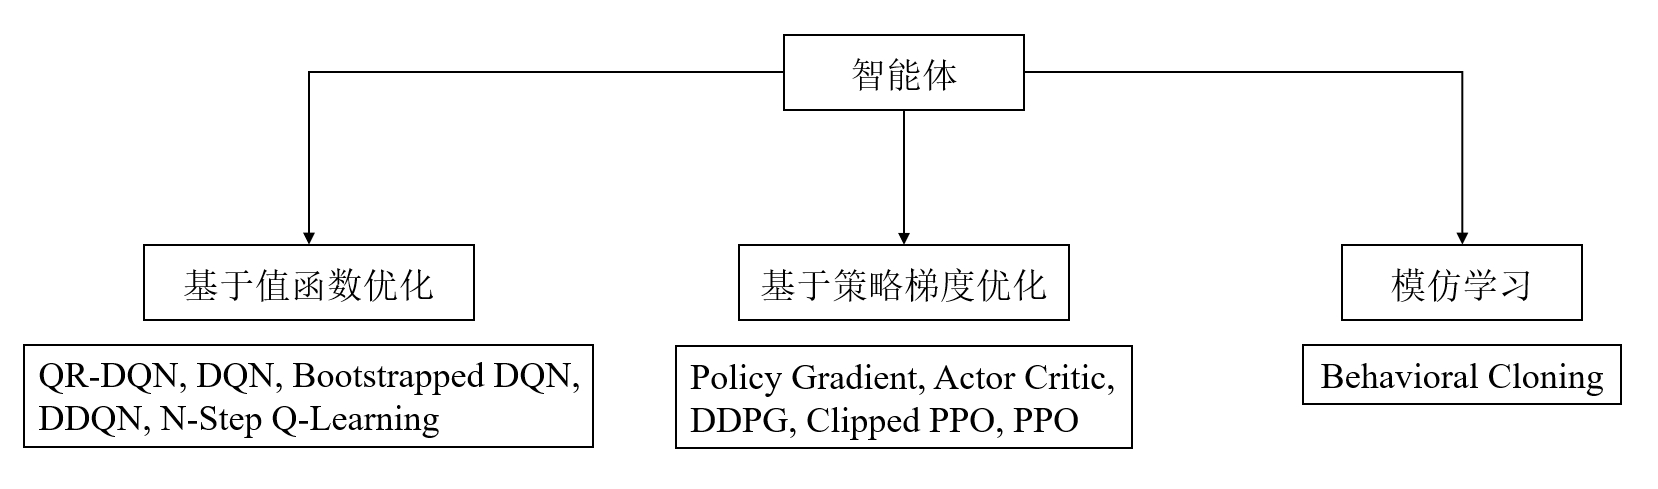
\includegraphics[width=15cm]{./pic/fg6.jpg}
		\caption{主流强化学习算法}
		\label{fg6}
	\end{figure}
	
	如图\ref{fg6}所示,目前主流的强化学习算法主要分为如下几类:
	\begin{enumerate}
		\item 基于值函数优化(Value Optimization)的算法,代表算法为Q-Learning,Mnih 等人将卷积神经网络与传统RL中的Q-Learning算法相结合,提出了深度Q网络(Deep Q-Network, DQN)模型,此后又涌现出双深度Q网络(Double Deep Q-Network, DDQN)、分类Q网络(Categorical Deep Q-Network,CDQN)、增强Q网络(Bootstrapped Deep Q-Network)等一系列值优化模型;
		
		\item 基于策略梯度优化(Policy Optimization)的算法,此类算法可以能够直接在策略空间中搜索最优策略,从而比基于值函数优化的方法实用性更广,代表算法有区域信赖的策略最优化方法(Trust Region Policy Optimization,TRPO)、近端梯度优化方法(Proximal Policy Optimization, PPO)。
		
		\item 行动者-评论者优化方法(Actor-Critic),Lillicrap 等人利用DQN扩展Q-Learning的思路对确定性梯度策略(Deterministic Policy Gradient,DPG)方法进行改造,提出了一种基于AC 框架的深度确定性策略梯度(Deep Deterministic Policy Gradient,DDPG)算法,并在解决连续动作空间问题上取得了很好的效果。
	\end{enumerate}
	
	\section{本文的主要贡献与创新}
	本文尝试将虚拟现实技术中的Unity 3D环境与强化学习算法的训练结合起来,使得强化学习的训练时间大幅度减少。同时通过Unity强大的物理引擎尽可能地拟合真实环境,从而使得训练出的强化学习模型无需经过细致调参优化就可以很好地迁移应用到实体机械环境上。
	
	\section{本论文的结构安排}
	本文的主要章节安排如下:第二章主要介绍了强化学习领域的基础知识,并对主流的强化学习算法的发展路线进行梳理;第三章首先介绍了Unity相对于传统强化学习仿真框架的优势,然后对本文采用的强化学习算法进行介绍,之后分别在2D环境和3D环境中实践该算法,并对Unity与强化学习整合的可能性进行评估;第四章对全文进行总结和回顾。
	
	\chapter{强化学习理论}
	\section{强化学习基础}
	RL是一种从环境状态映射到动作的学习,目标是使agent在与环境的交互过程中获得最大的累积奖赏。马尔可夫决策过程(Markov Decision Process,MDP)可以用来对RL问题进行建模。通常将MDP 定义为一个四元组$(S,A,\rho,f)$,其中:
	
	\begin{enumerate}
		\item $S$为所有环境状态的集合。$s_t\in S$表示agent在$t$时刻所处的状态;
		\item $A$为agent可执行动作的集合。$a_t\in A$表示agent在$t$时刻所采取的动作;
		\item $\rho:S\times A\rightarrow R$为奖赏函数。$r_t\sim \rho(s_t,a_t)$表示agent在状态执行动作获得的立即奖赏值;
		\item $f:S\times A\times S\rightarrow [0,1]$为状态转移概率分布函数。$S_{t+1}\sim f(s_t,a_t)$表示agent在状态$s_t$执行动作$a_t$转移到下一状态$S_{t+1}$的概率。
	\end{enumerate}
	
	在RL中,策略$\pi :S\rightarrow A$是状态空间到动作空间的一个映射。表示为agent在状态$s_t$选择动作$a_t$,执行该动作并以概率$f(s_t,a_t)$转移到下一状态$s_{t+1}$,同时接受来自环境反馈地奖赏$r_t$。假设未来每个时间步所获得的立即奖赏都必须乘以一个折扣因子$\gamma$,则从$t$时刻开始到$T$时刻结束时,奖赏之和定义为:
	\begin{equation}\label{eq1}
	R_t=\sum^T_{t'=t}\gamma^{t'-t}r_t
	\end{equation}
	
	其中$\gamma\in [0,1]$,用来权衡未来奖赏对累计奖赏的影响。
	状态动作值函数$Q^\pi (s,a)$指的是在当前状态$s$下执行该动作$a$,并一直遵循策略$\pi$到情节结束,这一过程中agent所获得的累计回报表示为:
	\begin{equation}\label{eq2}
	Q^\pi (s,a)=E[R_t|s_t=s,a_t=a,\pi]
	\end{equation}
	
	对于所有的状态动作对,如果一个策略$\pi ^*$的期望回报大于或等于其他所有策略的期望回报,那么称策略$\pi ^*$为最优策略。最优策略可能不只一个,但它们共享一个状态动作值函数:
	\begin{equation}\label{eq3}
	Q^\pi (s,a)=max_\pi E[R_t|s_t=s,a_t=a,\pi]
	\end{equation}
	
	式\ref{eq3}被称为最优状态值函数,且最优状态动作值函数遵循贝尔曼最优方程(Bellman Optimality Equation)。即:
	\begin{equation}
	\label{eq4}
	Q^*(s,a)=E_{s'\sim S}[r+\gamma max_{a'}Q(s',a')|s,a]
	\end{equation}
	
	在传统的RL中,一般通过迭代贝尔曼方程求解Q值函数:
	\begin{equation}
	\label{eq5}
	Q_{i+1}(s,a)=E_{s'\sim S}[r+\gamma max_{a'}Q_i(s',a')|s,a]
	\end{equation}
	
	其中,当$i\rightarrow\infty$时,$Q_i\rightarrow Q^*$。即通过不断地迭代会使状态动作值函数最终收敛,从而得到最优策略$\pi^*=argmax_{a\in A}Q^*(s,a)$。然而对于实际问题来说,通过迭代式\ref{eq5}求解最优策略显然是不可行的,因为在大状态空间下,用迭代贝尔曼方程求解$Q$值函数的方法计算代价太大.针对此问题,在RL算法中,通常使用线性函数逼近器来近似表示状态动作值函数,即$Q(s,a,\theta)\approx Q^*(s,a)$。此外,也可以用深度神经网络等非线性函数逼近器去近似表示值函数或策略。然而将RL与深度神经网络相结合可能会出现算法不稳定等问题,这一直阻碍着DRL的发展与应用。
	
	\section{基于值函数的深度强化学习}
	\subsection{深度Q网络}
	Mnih等人将卷积神经网络与传统RL中的Q学习算法相结合,提出了深度Q网络(Deep Q-Network, DQN)模型.该模型用于处理基于视觉感知的控制任务,是DRL领域的开创性工作.
	
	\subsubsection{模型结构}
	DQN模型的输入是距离当前时刻最近的4幅预处理后的图像。该输入经过3个卷积层和2个全连接层的非线性变换,最终在输出层产生每个动作的Q值。图\ref{fg1}表示DQN的模型结构。
	\begin{figure}
		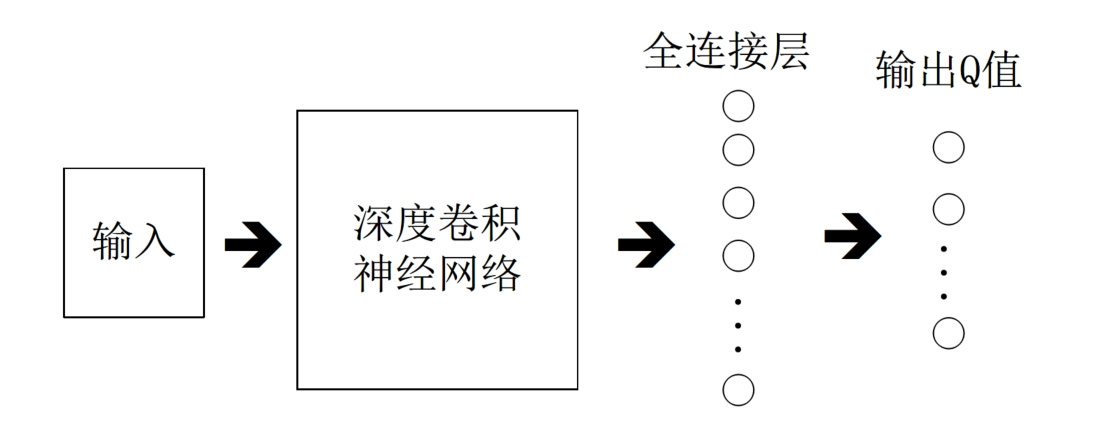
\includegraphics[width=8cm]{./pic/fg1.jpg}
		\caption{DQN的模型结构}
		\label{fg1}
	\end{figure}
	
	\subsubsection{训练算法}
	\begin{figure}
		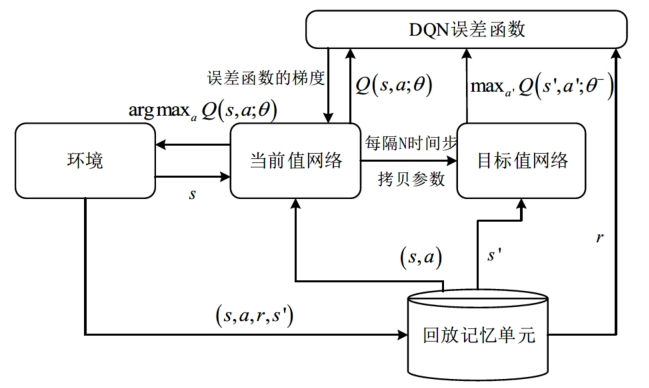
\includegraphics[width=10cm]{./pic/fg2.jpg}
		\caption{DQN的训练过程}
		\label{fg2}
	\end{figure}
	图\ref{fg2}描述了DQN的训练过程。为缓解非线性网络表示值函数时出现的不稳定等问题,DQN主要对传统的Q学习算法做了3处改进。
	
	\begin{enumerate}
		\item DQN在训练过程中使用经验回放机制(experience replay),在线处理得到的转移样本$e_t=(s_t,a_t,r_t,s_{t+1})$。在每个时间步$t$,将agent与环境交互得到的转移样本存储到回放记忆单元$D={e_1,...e_t}$中。训练时,每次从$D$中随机抽取小批量的转移样本,并使用随机梯度下降(Stochastic Gradient Descent, SGD)算法更新网络参数$\theta$。在训练深度网络时,通常要求样本之间是相互独立的。这种随机采样的方式,大大降低了样本之间的关联性,从而提升了算法的稳定性。
		
		\item DQN除了使用深度卷积网络近似表示当前的值函数之外,还单独使用了另一个网络产生目标Q值。具体地,$Q(s,a|\theta_i)$表示当前值网络的输出,用来评估当前状态动作对的值函数;$Q(s,a|\theta^-_i)$表示目标值网络的输出,一般采用近似表示值函数的优化目标,即目标Q值.当前值网络的参数$\theta$是实时更新的,每经过N轮迭代,将当前值网络的参数复制给目标值网络。通过最小化当前Q值和目标Q值之间的均方误差来更新网络参数,误差函数为:
		\begin{equation}
			\label{eq6}
			L(\theta_i)=E_{s,a,r,s'}[(Y_i-Q(s,a|\theta_i))^2]
		\end{equation}
		对参数$\theta$求偏导,得到一下梯度:
		\begin{equation}
			\label{eq7}
			\nabla_{\theta_i}=E_{s,a,r,s'}[(Y_i-Q(s,a|\theta_i))\nabla_{\theta_i}Q(s,a|\theta_i)]
		\end{equation}
		引入目标值网络后,在一段时间内目标Q值是保持不变的,一定程度上降低了当前Q值和目标Q值之间的相关性,提升了算法的稳定性。
		
		\item DQN将奖赏值和误差项缩小到有限的区间内,保证了Q值和梯度值都处于合理的范围内,提高了算法的稳定性。实验表明,DQN在解决诸如Atari 2600游戏等类真实环境的复杂问题时,表现出与人类玩家相媲美的竞技水平,甚至在一些难度较低的非战略性游戏中,DQN的表现超过了有经验的人类玩家。在解决各类基于视觉感知的DRL任务时,DQN使用了同一套网络模型、参数设置和训练算法,这充分说明DQN方法具有很强的适应性和通用性。
	\end{enumerate}

	\subsection{深度Q网络训练算法的改进}
	\subsubsection{深度双Q网络}\label{sec1}
	在DQN中使用$Y_i=r+\gamma max_{a'}Q(s',a'|\theta_i^-)$近似表示值函数的优化目标时,每次都选取下一个状态中最大Q值所对应的动作。选择和评价动作都是基于目标值网络的参数$\theta^-$,这会引起在学习过程中出现过高估计Q值的问题。
	
	Hasselt等人基于双Q学习算法(double Q-learning),提出了深度双Q网络(Deep DoubleQ-Network, DDQN)算法。在双Q学习中有两套不同的参数:$\theta$和$\theta^-$。其中$\theta$用来选择对应最大Q值的动作,$\theta$用来评估最优动作的Q值。两套参数将动作选择和策略评估分离开,降低了过高估计Q值的风险。因此DDQN使用当前值网络的参数$\theta$来选择最优动作,使用目标值网络的参数$\theta^-$来评估该最优动作。目标Q值的形式如下:
	\begin{equation}
		\label{eq8}
		Y_i^{DDQN}=r+\gamma Q(x',argmax_a Q(s',a'|\theta_i^-))
	\end{equation}
	DDQN在其他方面都与DQN保持一致。实验表明,DDQN能够估计出更加准确的Q值,在一些Atari 2600游戏中可获得更稳定有效的策略。
	
	\subsubsection{基于优势学习的深度Q网络}
	根据\ref{sec1}节可知,降低Q值的评估误差可以提升性能。Bellemare等人在贝尔曼方程中定义新的操作符,来增大最优动作值和次优动作值之间的差异,以缓和每次都选取下一状态中最大Q值对应动作所带来的评估误差。具体的改进如下:
	基于采样得到的样本计算均方误差$\Delta Q(s,a)^2$,其中误差项定义为:
	\begin{equation}
		\label{eq9}
		\Delta Q(s,a)=r+\gamma V(s')-Q(s,a)
	\end{equation}
	根据优势学习(Advantage Learning,AL)定义两种新的操作符,并将这两种操作符运用到上式中,分别得到AL误差项和一致性优势学习(Persistent Advantage Learning,PAL)误差项。其中AL误差项定义为:
	\begin{equation}
		\label{eq10}
		\Delta_{AL}Q(s,a)=\Delta Q(s,a)-\alpha[V(s)-Q(s,a)]
	\end{equation}
	为了定义PAL误差项,构造出如下式:
	\begin{equation}
		\label{eq11}
		\Delta_{AL}Q'(s,a)=\Delta Q(s',a)-\alpha[V(s)-Q(s',a)]
	\end{equation}
	得到PAL误差项的具体形式:
	\begin{equation}
		\label{eq12}
		\Delta_{PAL}Q(s,a)=max{\Delta_{AL}Q(s,a),\Delta_{AL}Q'(s,a)}
	\end{equation}
	实验表明,用AL和PAL误差项来替代贝尔曼方程中的误差项,可以有效地增加最优和次优动作对应值函数之间的差异,从而获得更加精确的Q值。即在DQN中加入AL和PAL误差项,可以有效地减小评估Q值时的偏差,促进学习效果的进一步提升,在许多Atari 2600游戏中取得了更好的表现。其中,采用PAL误差项时,最优和次优动作对应值函数之间的差异更大,Q值的评估也更加精确。
	
	\subsubsection{基于优先级采样的深度Q网络}
	DQN为了消除转移样本$e_t=(s_t,a_t,r_t,s_{t+1})$之间的相关性,使用经验回放机制在线地存储和使用agent与环境交互得到的历史样本。在每个时刻,经验回放机制从样本池中等概率地抽取小批量的样本用于训练。然而等概率采样并不能区分不同样本的重要性,同时由于样本池D的存储量有限,某些样本还未被充分利用就已经被舍弃。针对该问题,Schaul等人在DDQN的基础上提出了一种基于比例优先级采样的深度双Q网络(double deep Q-Network with proportional prioritization)。该方法用基于优先级的采样方式来替代均匀采样,提高一些有价值样本的采样概率,从而加快最优策略的学习。具体的改进如下:

	该抽样方法将每个样本的时间差分(Temporal Difference,TD)误差项作为评价优先级的标准。该误差为:$r+\gamma max_{a'}Q(s',a'|\theta^-)-Q(s,a|\theta)$,并且其绝对值越大,对应样本被采样的概率越高。在抽样过程中该方法使用随机比例化(stochastic prioritization)和重要性采样权重(importance-sampling weights)两种技巧。其中,随机比例化操作不仅能充分利用较大TD误差项对应的样本,而且保证了抽取样本的多样性。重要性采样权重的使用放缓了参数更新的速度,保证了学习的稳定性。实验表明,基于该抽样方式的深度双Q网络可以提升训练速度,并在很多Atari 2600游戏中获得了更高的分数。
	
	另外,Lakshminarayanan等人使用动态跳帧的方式来替代DQN中每个时刻重复k次的动作,提出了动态跳帧的DQN(Dynamic Frame Skip DeepQ-Network,DFDQN)算法。实验表明,DFDQN在一些Atari 2600游戏中取得了更好的性能;Hasselt等人使用一种称为Pop-Art的动态归一化操作来替代传统DQN中的区间裁剪方法。在不流失重要状态信息的前提下,统一了不同任务中目标Q值的量级,提高了agent在很多Atari2600游戏中的表现;Vincent等人在DQN中使用自适应的折扣因子和学习率,加速了深度网络收敛的速度。
	
	\subsection{DQN模型结构的改进}
	对DQN模型的改进一般是通过向原有网络中添加新的功能模块来实现的。例如,可以向DQN模型中加入循环神经网络结构,使得模型拥有时间轴上的记忆能力。本节主要介绍两种重要的DQN模型的改进版本,分别是基于竞争架构的DQN和深度循环Q网络(Deep Recurrent Q-Network,DRQN)。
	\subsubsection{基于竞争架构的DQN}
	在很多基于视觉感知的DRL任务中,受不同动作的影响,状态动作对的值函数是不同的。然而在某些状态下,值函数的大小是与动作无关的。利用上述思想,Wang等人设计了一种竞争网络结构(dueling network),并将其加入到DQN网络模型中。如图\ref{fg3},该网络结构与DQN模型的不同之处在于:DQN将CNN提取的抽象特征经过全连接层后,直接在输出层输出对应动作的Q值,而引入竞争网络结构的模型则将CNN提取的抽象特征分流到两个支路中,其中一路代表状态值函数,另一路代表依赖状态的动作优势函数(advantage function)。通过该种竞争网络结构,agent可以在策略评估过程中更快地识别出正确的行为。
	\begin{figure}
		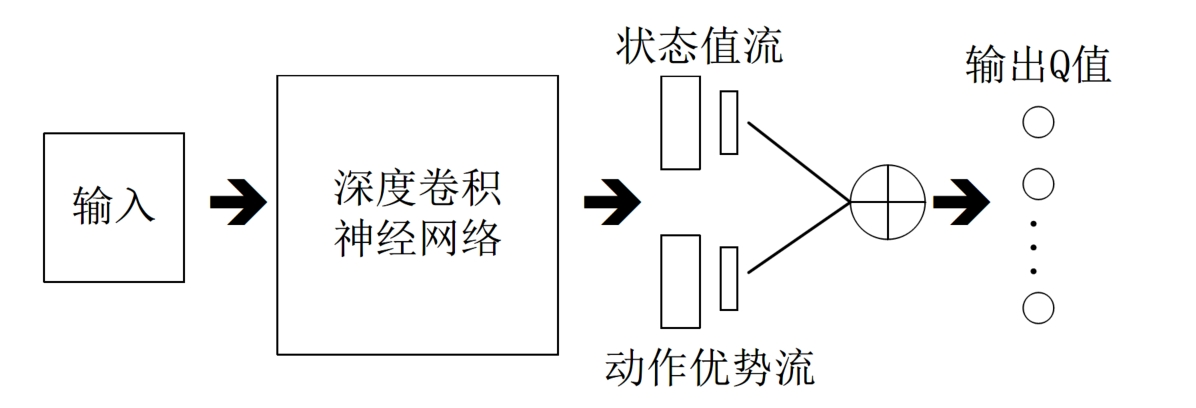
\includegraphics[width=8cm]{./pic/fg3.jpg}
		\caption{基于竞争架构的DQN模型结构}
		\label{fg3}
	\end{figure}
	具体地,状态值函数表示为$\hat{V}(s|\theta,\beta)$,动作优势函数表示为$\hat{A}(s,a|\theta,\alpha)$。通过一种聚合操作将状态值流和动作优势流相结合:
	\begin{equation}
		\label{eq13}
		Q(s,a|\theta,\alpha,\beta)=\hat{V}(s|\theta,\beta)+\hat{A}(s,a|\theta,\alpha)
	\end{equation}
	其中,$\alpha$、$\beta$和$\theta$分别代表状态值流、动作优势流和模型剩余部件的参数。然而在实际操作中,一般要将动作优势流设置为单独动作优势函数值减去某状态下所有动作优势函数的平均值。该技巧不仅可以保证该状态下各动作的优势函数相对排序不变,而且可以缩小Q值的范围,去除多余的自由度。实验表明,在DQN中加入竞争网络可以使得值函数的估计更加精确。在频繁出现agent采取不同动作但对应值函数相等的情形下,竞争架构的DQN模型性能提升最为明显。
	
	\subsubsection{深度循环Q网络}
	在传统的RL方法中,状态信息的部分可观察性一直是个亟待解决的难题。DQN通过堆叠离当前时刻最近的4幅历史图像组成输入状态,有效缓解了状态信息的部分可观察问题,却增加了网络的计算和存储负担。针对此问题,Hausknecht等人利用循环神经网络结构来记忆时间轴上连续的历史状态信息,提出了DRQN模型。
	\begin{figure}
		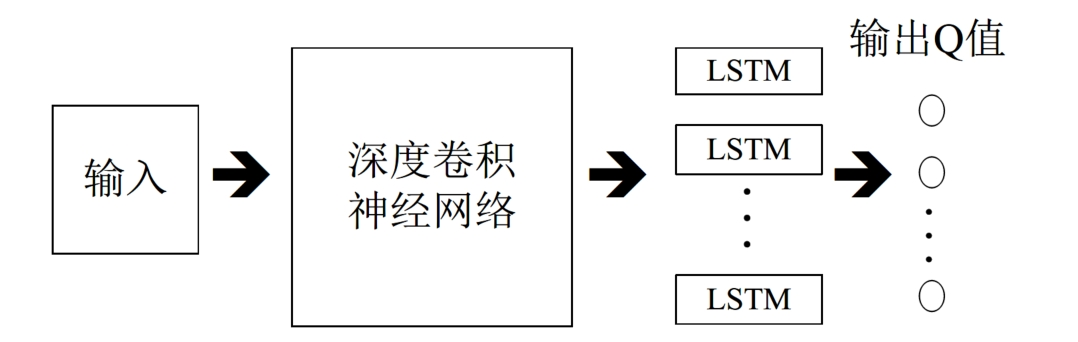
\includegraphics[width=8cm]{./pic/fg4.jpg}
		\caption{DRQN模型结构}
		\label{fg4}
	\end{figure}
	如图\ref{fg4}所示,DRQN将DQN中第1个全连接层的部件替换成了256个长短期记忆单元(Long Short-TermMemory,LSTM)。此时模型的输入仅为当前时刻的一幅图像,减少了深度网络感知图像特征所耗费的计算资源。实验表明,在部分状态可观察的情况下,DRQN表现出比DQN更好的性能。因此DRQN模型适用于普遍存在部分状态可观察问题的复杂任务。
	
	随着DL领域中各种新颖网络模块的提出,未来DRL模型会朝着结构多样化、模块复杂化的方向发展。例如,可以利用深度残差网络所具备的强大感知能力来提高agent对复杂状态空间的表征效果;另外,可以在模型中加入视觉注意力机制(Visual Attention Mechanism,VAM),使得agent在不同状态下将注意力集中到有利于做出决策的区域,从而加速学习的进程。
	
	\section{基于策略梯度的深度强化学习}
	策略梯度是一种常用的策略优化方法,它通过不断计算策略期望总奖赏关于策略参数的梯度来更新策略参数,最终收敛于最优策略。因此在解决DRL问题时,可以采用参数为的深度神经网络来进行参数化表示策略,并利用策略梯度方法来优化策略。值得注意的是,在求解DRL问题时,往往第一选择是采取基于策略梯度的算法。原因是它能够直接优化策略的期望总奖赏,并以端对端的方式直接在策略空间中搜索最优策略,省去了繁琐的中间环节。因此与DQN及其改进模型相比,基于策略梯度的DRL方法适用范围更广,策略优化的效果也更好。
	\subsection{深度策略梯度的起源与发展}\label{sec2}
	策略梯度方法是一种直接使用逼近器来近似表示和优化策略,最终得到最优策略的方法。该方法优化的是策略的期望总奖赏:
	\begin{equation}
		\label{eq14}
		max_{\theta}E[R|\pi_\theta]
	\end{equation}
	其中$R=\sum_{t=0}^{T-1}$表示一个情节内所获得的奖赏总和。策略梯度最常见的思想是增加总奖赏较高情节出现的概率。策略梯度方法的具体过程如下:
	假设一个完整情节的状态、动作和奖赏的轨迹为:$\tau=(s_0,a_0,r_0,s_1,a_1,r_1,...,s_{T-1},a_{T-1},r_{T-1},s_T)$。则策略梯度表示为如下的形式:
	\begin{equation}
		\label{eq15}
		g=R\nabla_\theta\sum_{t=0}^{T-1}log\pi(a_t|s_t;\theta)
	\end{equation}
	利用该梯度调整策略参数:
	\begin{equation}
		\label{eq16}
		\theta\leftarrow\theta+\alpha g
	\end{equation}
	其中,$\alpha$是学习率,控制着策略参数更新的速率。式\ref{eq15}中的$\nabla_\theta\sum_{t=0}^{T-1}log\pi(a_t|s_t;\theta)$梯度项表示能够提高轨迹$\tau$出现概率的方向,乘以得分函数R之后,可以使得单个情节内总奖赏越高的$\tau$概率密度越大。即如果收集了很多总奖赏不同的轨迹,通过上述训练过程会使得概率密度向总奖赏更高的轨迹方向移动,最大化高奖赏轨迹$\tau$出现的概率。
	然而在某些情形下,每个情节的总奖赏R都不为负,那么所有梯度g的值也都是大于等于0的。此时在训练过程中遇到每个轨迹$\tau$,都会使概率密度向正的方向“拉拢”,很大程度减缓了学习速度。这会使得梯度g的方差很大。因此可以对R使用某种标准化操作来降低梯度g的方差。该技巧使得算法能提高总奖赏R较大的轨迹$\tau$的出现概率,同时降低总奖赏R较小的轨迹$\tau$出现概率。根据上述思想,Williams等人提出了REINFORCE算法,将策略梯度的形式统一为:
	\begin{equation}
		\label{eq17}
		g=\nabla_\theta\sum_{t=0}^{T-1}log\pi(a_t|s_t;\theta)(R-b)
	\end{equation}
	其中,b是一个与当前轨迹$\tau$相关的基线,通常设置为R的一个期望估计,目的是减小R的方差。可以看出,R超过基准b越多,对应的轨迹$\tau$被选中的概率越大。因此在大规模状态的DRL任务中,可以通过深度神经网络参数化表示策略,并采用传统的策略梯度方法来求解最优策略。
	
	此外,优化策略的另一种思路是增加“好”的动作出现的概率。在RL中一般是通过优势函数评价动作的好坏,因此可以利用优势函数项来构造策略梯度:
	\begin{equation}
		\label{eq18}
		g=\nabla_\theta\sum_{t=0}^{T-1}\hat{A}log\pi(a_t|s_t;\theta)
	\end{equation}
	其中$\hat{A_t}$表示状态动作对$(s_t,a_t)$优势函数的一个估计,通常构造成以下形式:
	\begin{equation}
		\label{eq19}
		\hat{A_t^\gamma}=r_t+\gamma r_{t+1}+\gamma^2 r_{t+2}+\dots-V(s_t)
	\end{equation}
	其中,$\gamma\in[0,1]$表示折扣因子。此时带折扣的奖赏之和$r_t+\gamma r_{t+1}+\gamma^2 r_{t+2}+\dots$相当于式\ref{eq17}中的R,带折扣的状态值函数$V(s_t)$相当于式\ref{eq17}中的基准$b$。当$\hat{A_t^\gamma}>0$时,会增加对应动作被选择的概率,而当$\hat{A_t^\gamma}<0$,会减少对应动作被选择的概率。
	
	另外,Hafner等人使用值函数来估计带折扣的奖赏和,进一步地缩小了梯度项地方差。此时进一步截断的$\hat{A_t^\gamma}$表示为:
	\begin{equation}
		\label{eq20}
		\hat{A_t^\gamma}=r_t+\gamma V(s_{t+1})-V(s_t)
	\end{equation}
	类似地,两步截断的$\hat{A_t^\gamma}$表示为:
	\begin{equation}
		\label{eq21}
		\hat{A_t^\gamma}=r_t+\gamma r_{t+1}+\gamma^2V(s_{t+2})-V(s_t)
	\end{equation}
	然而使用值函数估计带折扣的奖赏和,也会产生一定的估计偏差。为了缩小方差的同时还能保证偏差较小,Schulman等人提出了广义优势函数(generalized advantage function):
	\begin{equation}
		\label{eq22}
		\hat{A_t^\gamma}=\delta_t+(\gamma\lambda)\delta_{t+1}+\dots+(\gamma\lambda)^{T-t-1}\delta_{T-1}
	\end{equation}
	其中$\delta_t=r_t+\gamma r_{t+1}+\gamma^2V(s_{t+2})-V(s_t)$。$\lambda$是一个调节因子,范围大小为$0<\lambda<1$。当$\lambda$接近0时,$\hat{A_t^\gamma}$是低方差、高误差的;当$\lambda$接近于1时,$\hat{A_t^\gamma}$是高方差、低误差的。
	
	基于广义优势函数的策略梯度方法的不足之处在于:在利用式\ref{eq16}全局优化策略的过程中,很难确定一个合理的步长参数$\alpha$来保证学习的稳定性。针对此问题,Schulman\cite{Schulman2015Trust}等人提出了一种被称为区域信赖的策略最优化(Trust Region Policy Optimization,)方法。TRPO的核心思想是:强制限制同一批次数据上新旧两种策略预测分布的KL差异,从而避免导致策略发生太大改变的参数更新步。为了将应用范围扩展到大规模状态空间的DRL任务中,TRPO算法使用深度神经网络来参数化策略,在只接收原始输入图像的情况下实现了端对端的控制。实验表明,TRPO在一系列2D场景下的机器人控制和Atari 2600游戏任务中都表现优异。此后,Schulman等人又尝试将广义优势函数与TRPO方法相结合,在一系列3D场景下的机器人控制任务中取得了突破。
	
	此外,深度策略梯度方法的另一个研究方向是通过增加额外的人工监督来促进策略搜索。例如著名的AlphaGo围棋机器人,先使用监督学习从人类专家的棋局中预测人类的走子行为,再用策略梯度方法针对赢得围棋比赛的真实目标进行精细的策略参数调整。然而在某些任务中是缺乏监督数据的,比如现实场景下的机器人控制,可以通过引导式策略搜索(guided policy search)方法来监督策略搜索的过程。在只接受原始输入信号的真实场景中,引导式策略搜索实现了对机器人的操控。
	
	\subsection{基于行动者评论家的深度策略梯度方法}
	\ref{sec2}节中深度策略梯度方法的基本思想是通过各种策略梯度方法直接优化用深度神经网络参数化表示的策略。这类方法在每个迭代步,都需要采样批量大小为N的轨迹${\tau_i}^N_{i=1}$来更新策略梯度。然而在许多复杂的现实场景中,很难在线获得大量训练数据。例如在真实场景下机器人的操控任务中,在线收集并利用大量训练数据会产生十分昂贵的代价,并且动作连续的特性使得在线抽取批量轨迹的方式无法达到令人满意的覆盖面。以上问题会导致局部最优解的出现。针对此问题,可以将传统RL中的行动者评论家(Actor-Critic,AC)框架拓展到深度策略梯度方法中。图\ref{fg5}展示了基于AC框架的深度策略梯度方法的学习结构。
	\begin{figure}
		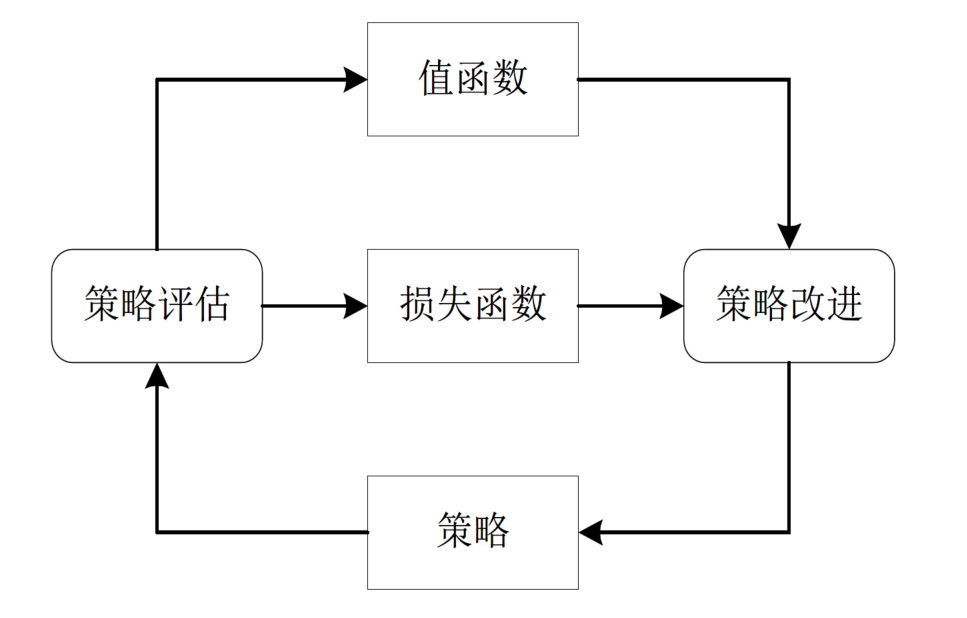
\includegraphics[width=8cm]{./pic/fg5.jpg}
		\caption{基于AC框架的深度策略梯度方法的学习结构}
		\label{fg5}
	\end{figure}

	下面阐述一种重要的基于AC框架的深度策略梯度算法。Lillicrap等人利用DQN扩展Q学习算法的思路对确定性策略梯度(Deterministic Policy Gradient,DPG)方法进行改造,提出了一种基于AC框架的深度确定性策略梯度(Deep Deterministic Policy Gradient,DDPG)算法,该算法可用于解决连续动作空间上的DRL问题。DDPG分别使用参数为$\theta^\mu$和$\theta^Q$的深度神经网络来表示确定性策略$a=\pi(s|\theta^\mu)$和值函数$Q(s,a|\theta^Q)$。其中,策略网络用来更新策略,对应AC框架中的行动者;值网络用来逼近状态动作对的值函数,并提供梯度信息,对应AC框架中的评论家。在DDPG中,目标函数被定义为带折扣的奖赏和:
	\begin{equation}
		\label{eq23}
		J(\theta^\mu)=E_{\theta^\mu}[r_1+\gamma r_2+\gamma^2r_3+\dots]
	\end{equation}
	然后,采用随机梯度下降方法来对目标函数进行端对端的优化。Silver等人证明了目标函数关于$\theta^\mu$的梯度等价于Q值函数关于$\theta^\mu$的期望梯度:
	\begin{equation}
		\label{eq24}
		\frac{\partial J(\theta^\mu)}{\partial \theta^\mu}=E_s[\frac{\partial Q(s,a|\theta^Q)}{\partial \theta^\mu}]
	\end{equation}
	根据确定性策略$a=\pi(s|\theta^\mu)$可得:
	\begin{equation}
		\label{eq25}
		\frac{\partial J(\theta^\mu)}{\partial \theta^\mu}=E_s[\frac{\partial Q(s,a|\theta^Q)}{\partial a}\frac{\partial \pi(s|\theta^\mu)}{\partial \theta^\mu}]
	\end{equation}
	通过DQN中更新值网络的方法来更新评论家网络,此时的梯度信息为:
	\begin{equation}
		\label{eq26}
		\frac{\partial J(\theta^Q)}{\partial \theta^Q}=E_{s,a,r,s'\sim D}[(y-Q(s,a|\theta^Q))\frac{\partial Q(s,a|\theta^Q)}{\partial \theta^Q}]
	\end{equation}
	其中,$y=r+\gamma Q(s',\pi(s'|\hat{\theta ^\mu})|\hat{\theta ^Q})$,$\hat{\theta ^\mu}$和$\hat{\theta ^Q}$分别表示目标策略网络和目标值网络的参数。DDPG使用经验回放机制从D中获得训练样本,并将由Q值函数关于动作的梯度信息从评论家网络传递给行动者网络。并根据式\ref{eq25}沿着提升Q的方向更新策略网络的参数。
	
	实验表明,DDPG不仅在一系列连续动作空间的任务中表现稳定,而且求得最优解所需要的时间步也远远少于DQN。与基于值函数的DRL方法相比,基于AC框架的深度策略梯度方法优化策略效率更高、求解速度更快。
	
	然而在有噪声干扰的复杂环境下,策略一般都具有一定的随机性。DDPG使用确定性的策略梯度方法。对于随机环境的场景,该方法并不适用。针对此问题,Heess等人提出了一种适用于连续动作空间任务的通用框架,称为随机值梯度(Stochastic Value Gradient,SVG)方法。SVG使用“再参数化”(re-parameterization)的数学技巧来学习环境动态性的生成模型,将确定性策略梯度方法扩展为一种随机环境下的策略优化过程。Balduzzi等人基于相容的值函数逼近器(compatible function approximation)理论,提出了值梯度反向更新(Value-Gradient Backpropagation,GProp)方法。Peng等人融合多个策略网络和对应的值网络,提出了一种基于混合型行动者评论家指导(Mixture of Actor Critic Experts,MACE)的深度策略梯度方法。该方法在自适应机器人控制任务中取得了实质性的进展。MACE相比于单个AC框架指导的深度策略梯度方法,有着更快的学习速度。随后,Heess等人使用循环神经网络,进一步扩展了DPG和SVG算法的适用范围,提出了循环确定性策略梯度(Recurrent Deterministic Policy Gradient,RDPG)和循环随机值梯度(Recurrent Stochastic Value Gradient,RSVG)方法。RDPG和RSVG可以处理一系列部分可观察场景下连续动作的控制任务。Hausknecht等人进一步将深度策略梯度方法扩展到了参数化的连续动作空间问题中。此后,Schulman等人提出了一种形式化的随机计算图模型(stochastic computation graphs),开展了同时包含随机性和确定性操作的复杂深度策略梯度的研究。
	
	\subsection{异步优势行动者评论家算法}
	不同类型的深度神经网络为DRL中策略优化任务提供了高效运行的表征形式。为了缓解传统策略梯度方法与神经网络结合时出现的不稳定性,各类深度策略梯度方法(如DDPG、SVG等)都采用了经验回放机制来消除训练数据间的相关性。然而经验回放机制存在两个不足之处:
	\begin{enumerate}
		\item agent与环境的每次实时交互都需要耗费很多的内存和计算力;
		\item 经验回放机制要求agent采用离策略(off-policy)方法来进行学习,而离策略方法只能基于旧策略生成的数据进行更新。
	\end{enumerate}
	针对这些问题,Mnih等人根据异步强化学习(Asynchronous Reinforcement Learning,ARL)的思想,提出了一种轻量级的DRL框架,该框架可以使用异步的梯度下降法来优化网络控制器的参数,并可以结合多种RL算法。其中,异步的优势行动者评论家算法(Asynchronous Advantage Actor-Critic,A3C)在各类连续动作空间的控制任务上表现的最好。
	
	具体地,A3C算法利用CPU多线程的功能并行、异步地执行多个agent。因此在任意时刻,并行的agent都将会经历许多不同的状态,去除了训练过程中产生的状态转移样本之间的关联性。因此这种低消耗的异步执行方式可以很好地替代经验回放机制。
	
	A3C算法在训练时降低了对硬件的要求。深度策略梯度算法十分依赖计算能力很强的图形处理器(Graphics Processing Unit,GPU),而A3C算法在实际的操作过程中只需要一个标准的多核CPU。由表\ref{tb1}可知,A3C算法通过应用多线程技术,降低了模型对硬件的需求,在训练时间更少的情况下,A3C算法在Atari 2600游戏任务上的平均性能有明显提升。而且A3C算法能够只根据原始的视觉输入学习到行走3D迷宫的有效策略。此外,A3C算法还可以广泛应用于各种连续动作空间问题。综上所述,A3C算法能够广泛应用于各种2D、3D离散和连续动作空间的任务,并且在这些任务中都取得了最佳的效果。这说明A3C是目前最通用和最成功的一种DRL算法。当然,将A3C与近期的一些深度策略梯度算法相结合可能会进一步提升其性能。
	
	\begin{table}[h]
		\caption{不同的DRL模型在57个Atari游戏上的平均耗时以及游戏性能的提升}
		\label{tb1}
		\begin{tabular}{cccc}
			\toprule[1.5pt]
			模型 & 训练条件 & 训练时间/天 & 平均性能提升 \\
			\hline
			DQN & GPU & 8 & 121.9\% \\
			DDQN & GPU & 8 & 332.9\% \\
			Dueling DDQN & GPU & 8 & 343.8\% \\
			Prioritized DQN & GPU & 8 & 463.6\% \\
			A3C,FF & CPU & 1 & 344.1\% \\
			A3C,FF & CPU & 4 & 496.8\% \\
			A3C,LSTM & CPU & 4 & 623.0\% \\
			\bottomrule[1.5pt]
		\end{tabular}
	\end{table}
	除了基于值函数的DRL和基于策略梯度的DRL之外,还可以通过增加额外的人工监督来促进策略搜索的过程,即为基于搜索与监督的DRL的核心思想。蒙特卡洛树搜索(Monte Carlo Tree Search,MCTS)作为一种经典的启发式策略搜索方法,被广泛用于游戏博弈问题中的行动规划。因此在基于搜索与监督的DRL方法中,策略搜索一般是通过MCTS来完成的。例如Google公司的AlphaGo围棋算法就将深度神经网络和MCTS相结合,并取得了卓越的成就。
	
	\section{近端梯度优化算法}\label{ppo}
	\subsection{算法思路}\label{ppocontent}
	传统策略梯度算法存在一个两难问题:在更新策略参数时,需要确定更新步长(即学习率),如果步长过小,则更新速度过慢,时间开销将会难以忍受;而如果步长过大,学习到的策略效果过差,继续在此策略中进一步采样数据进行训练,会使策略的效果越来越差,引起恶性循环。因此,如何确定合适的梯度更新步长,是一个亟待解决的问题。为了解决此问题,TRPO算法强制限制同一批次数据上新旧两种预测分布的KL差异,从而避免导致策略发生太大改变,并提出了以下目标函数:
	\begin{equation*}
	\begin{aligned}
		& \underset{\theta}{\text{maximize}}& & \hat{E}_t[\frac{\pi_\theta(a_t|s_t)}{\pi_{\theta_{old}}(a_t|s_t)}\hat{A_t}]\\
		& \text{subject to }& &\hat{E}_t[KL[\pi_{\theta_{old}}(\cdot|s_t),\pi_\theta(\cdot|s_t)]]\leq \delta
	\end{aligned}
	\end{equation*}
	使用KL散度来描述新旧策略的差异,当差异在$\delta$表示的置信域范围内时,最大化目标表达式。其中$\theta_{old}$表示旧策略,$\hat{A}_t$表示采样样本的优势估计值,在进行优化时,先使用旧策略在环境中采样得到数据(包括状态、动作、奖励值等),然后在这些数据中多次随机采样得到小批量数据(minibatch),使用小批量数据优化策略函数。
	
	TRPO算法虽然有效地解决了更新步长问题,但由于约束条件需要计算一个二阶梯度(二阶海森矩阵),当目标函数的变量维度较高时,计算量会特别大,由此导致效率过低。而且TRPO算法无法兼容深度网络中的随机失活单元(dropout)以及进行参数共享(策略函数与值函数之间往往会共享参数)。
	
	因此,Schulman等人\cite{Schulman2017Proximal}又提出了近端策略优化方法(Proximal Policy Optimization Algorithms, PPO),该算法对TRPO算法进行了改进,相对于TRPO算法而言,PPO算法更易于实现,而且效率更高。TRPO算法并没有使用惩罚项来代替约束条件来保证策略更新的稳定性,原因是如果在最优化问题中引入惩罚项,
	\begin{equation}
		\label{eq27}	
		\underset{\theta}{\text{maximize }} \hat{E}_t[\frac{\pi_\theta(a_t|s_t)}{\pi_{\theta_{old}}(a_t|s_t)}\hat{A_t}]-\beta KL[\pi_{\theta_{old}}(\cdot|s_t),\pi_\theta(\cdot|s_t)]
	\end{equation}
	上式中的权重因子$\beta$将难以确定,不仅无法找到一个合适的$\beta$使其在多种任务中都取得良好效果,就连在单个任务中也无法找到合适的$\beta$值。
	
	于是PPO算法尝试使用一阶优化的方法来求解该问题,PPO算法提出了一个基于裁剪概率比率(clipped probability ratio)的目标函数。首先定义裁剪概率比率$r_t(\theta)=\frac{\pi_\theta(a_t|s_t)}{\pi_{\theta_{old}}(a_t|s_t)}$,即$r(\theta_{old})=1$,则TRPO中的目标函数可以表示为:
	\begin{equation}
		\label{eq28}
		L^{CPI}(\theta)=\hat{E}_t[\frac{\pi_\theta(a_t|s_t)}{\pi_{\theta_{old}}(a_t|s_t)}]=\hat{E}[r_t(\theta)\hat{A_t}]
	\end{equation}
	由于式\ref{eq28}中的策略更新有可能会特别大,因此PPO算法对其进行了改进,加入了裁剪项:
	\begin{equation}
		\label{eq29}
		L^{CLIP}(\theta) = \hat{\mathbb{E}}_t [\min(r_t(\theta) \hat{A}_t, \text{clip}(r_t(\theta), 1 - \epsilon, 1+\epsilon) \hat{A}_t)]
	\end{equation}
	其中$\epsilon$为超参数。其中的裁剪项使得$r_t$不偏离$[1-\epsilon, 1+\epsilon]$的区间,即当策略更新幅度大于预定区间时,裁剪项将对其幅度进行限制。
	
	除了基于裁剪概率比率的函数,PPO算法还提出了一种基于自适应KL惩罚系数的实现方案,对于式\ref{eq27}中提出的目标函数,其参数$\beta$可以采用以下方式动态调整:计算$d=\hat{E_t}[KL[\pi_{\theta_{old}}(\cdot|s_t), \pi_\theta(\cdot|s_t)]]$,如果$d<d_{target}/1.5$,$\beta\leftarrow\beta/2$;如果$d>d_{target}\times1.5$,$\beta\leftarrow\beta\times2$。
	
	目前PPO算法是OpenAI的强化学习基准算法集(baselines)的默认算法,它仅仅通过一个简单的裁剪机制,就解决了TRPO算法中二次梯度计算量过大、数据采样效率低等问题,并且大大提升了鲁棒性。
	
	因此,本文将采用PPO算法作为强化学习的代表算法,将Unity环境整合到PPO算法的训练过程中,并将对训练效果进行评估。
	
	\subsection{训练过程}
	PPO算法中,数据采样与优化交替进行,传统的策略梯度方法,每进行一次数据采样都要执行一次优化,而PPO算法则先进行多次数据采样,然后从采样得到的数据中随机抽取小批量数据,然后再执行优化。算法的训练过程如\ref{al1}所示。
	
	\begin{algorithm}[H]
		\caption{近端策略优化算法(动态调整$\lambda$版本)}
		\label{al1}
		\For{$i\in{1, \dots, N}$}{
			在$T$个时间步内执行策略$\pi_\theta$,收集采样数据${s_t, a_t, r_t}$\\
			评估优势$\hat{A_t}=\sum_{t'>t}\gamma^{t'-t}r_{t'}-V_\phi(s_t)$\\
			更新策略$\pi_{old}\leftarrow\pi_\theta$\\
			\For{$j\in{1, \dots, M}$}{
				$J_{PPO}(\theta)=\sum_{t=1}^{T}\frac{\pi_\theta(a_t|s_t}{\pi_{old}(a_t|s_t)}\hat{A_t}-\lambda KL[\pi_{old}|\pi_\theta]$\\
				根据目标函数$J_{PPO}(\theta)$更新$\theta$
			}
			\For{$j\in{1, \dots, B}$}{
				$L_{BL}(\phi)=-\sum_{t=1}^{T}(\sum_{t'>t}\gamma^{t'-t}r_{t'}-V_\phi(s_t))^2$\\
				根据目标函数$L_{BL}(\phi)$更新$\phi$
			}
			\If{$KL[\pi_{old}|\pi_\theta]>\beta_{high}KL_{target}$}{
				更新$\lambda\leftarrow\alpha\lambda$
			}
			\ElseIf{$KL[\pi_{old}|\pi_\theta]<\beta_{low}KL_{target}$}{
				更新$\lambda\leftarrow\frac{\lambda}{\alpha}$
			}
		}
	\end{algorithm}
	
	PPO算法是典型的行动者评论家架构,在训练过程中,行动者要最大化目标函数$J_{PPO}(\theta)$,评价者则要最小化误差$L_{BL}(\phi)$(Temporal-difference Error, TD Error)。同时$J_{PPO}(\theta)$中的超参数$\lambda$按照\ref{ppocontent}节中所述进行动态调整,从而使算法的性能达到最佳。
	
	\begin{algorithm}[H]
		\caption{近端策略优化算法(裁剪概率比值版本)}
		\label{al2}
		\For{$i\in{1, \dots, N}$}{
			在$T$个时间步内执行策略$\pi_\theta$,收集采样数据${s_t, a_t, r_t}$\\
			评估优势$\hat{A_t}=\sum_{t'>t}\gamma^{t'-t}r_{t'}-V_\phi(s_t)$\\
			更新策略$\pi_{old}\leftarrow\pi_\theta$\\
			\For{$j\in{1, \dots, M}$}{
				$J_{PPO}(\theta)=\sum_{t=1}^{T}\frac{\pi_\theta(a_t|s_t}{\pi_{old}(a_t|s_t)}\hat{A_t}-\lambda KL[\pi_{old}|\pi_\theta]$\\
				根据目标函数$J_{PPO}(\theta)$更新$\theta$
			}
			\For{$j\in{1, \dots, B}$}{
				$L_{CLIP}(\theta) = \hat{\mathbb{E}}_t [\min(r_t(\theta) \hat{A}_t, \text{clip}(r_t(\theta), 1 - \epsilon, 1+\epsilon) \hat{A}_t)]$\\
				根据目标函数$L_{CLIP}(\phi)$更新$\phi$
			}
		}
	\end{algorithm}
	算法\ref{al2}是对\ref{al1}的改进版本,因为\ref{al1}引入的惩罚项系数$\lambda$十分难确定,即使使用了\ref{al1}中的自适应算法,效果也不尽如人意,而裁剪概率比值版本的效果则相对好得多,这一点将会在后续的实验部分进行验证。
	
	\chapter{强化学习算法实践}
	\section{强化学习常用仿真环境对比}
	\subsection{OpenAI Gym工具集}
	OpenAI是一个非营利性质的人工智能公司,其致力于有益于人类的友好型AI。Gym是该公司推出的一套工具集,用于为强化学习算法提供一个通用的评价标准。该工具集不对用户的agent做出任何限制,这导致该工具集有着极强的兼容性,可以很好地兼容诸如Tensorflow、Theano或者Keras等主流机器学习库。
	
	\begin{figure}[h]
		\centering
		\subfigure{
			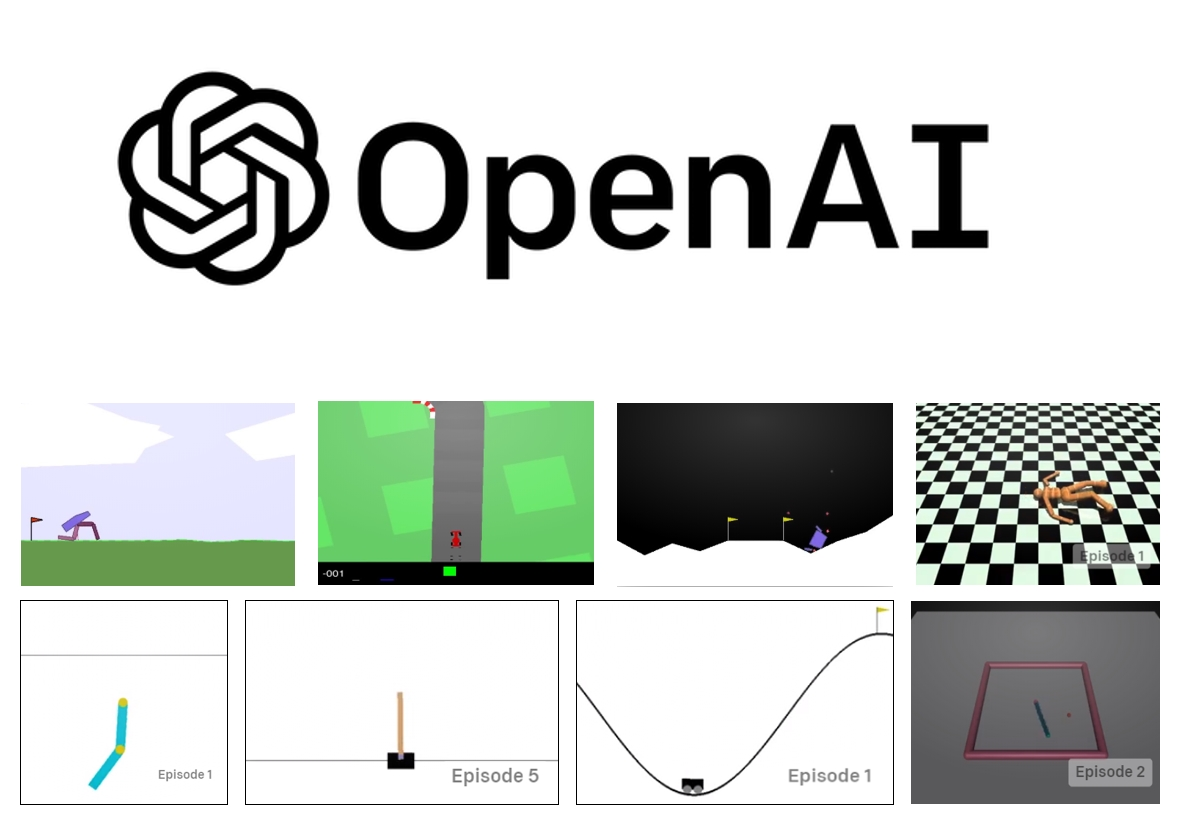
\includegraphics[width=7cm]{./pic/gym-envs.jpg}
		}
		\subfigure{
			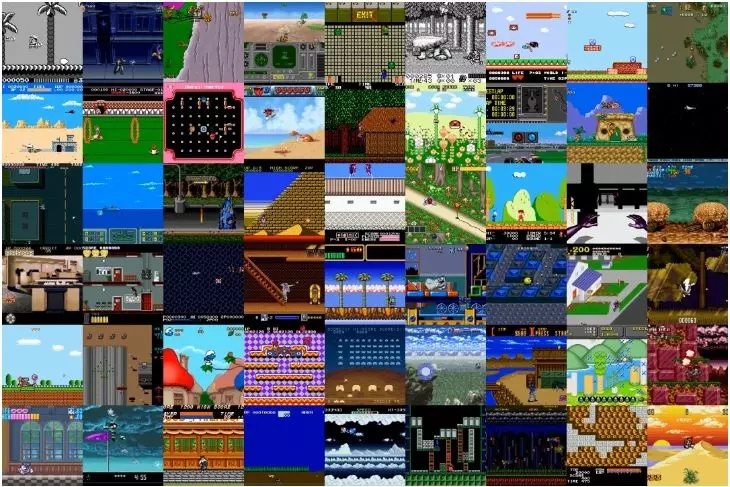
\includegraphics[width=7cm]{./pic/gym-game.jpg}
		}
		\caption{Gym内置了多种多样的环境}
		\label{openai}
	\end{figure}
	
	Gym工具集内置了多样化的测试环境,用户可以很方便地在这些环境中开发以及测试强化学习算法,这些环境共用同一套接口,这意味着用户可以用其编写通用性很强的算法。
	
	如\ref{openai}所示,目前Gym已经包含了摆臂、自动驾驶汽车、简单机械臂、蜘蛛型机器人、人形机器人等环境,不仅如此,Gym还包含了一个用于测试强化学习算法的游戏平台,涵盖了70余个雅达利和30多个世嘉平台游戏,并且OpenAI还发布了用于向Gym平台添加新游戏的工具。
	
	Gym极大地方便了学术界对强化学习算法及其泛化能力的研究,以往RL领域的研究主要集中在优化agent完成单个任务的能力上。
	
	\subsection{Robot Operating System(ROS)平台}
	ROS(Robot Operating System, 机器人操作系统),是专为机器人软件开发所设计出来的一套电脑操作系统架构。它是一个开源的元级操作系统(后操作系统),提供类似于操作系统的服务,包括硬件抽象描述、底层驱动程序管理、共用功能的执行、程序间消息传递、程序发行包管理,它也提供一些工具和库用于获取、建立、编写和执行多机融合的程序。
	
	ROS的运行架构是一种使用ROS通信模块实现模块间P2P(Peer to Peer, 点对点)的松耦合的网络连接的处理架构,它执行若干种类型的通讯,包括:
	\begin{itemize}
		\item 基于服务的同步RPC(Remote Progress Call, 远程过程调用)通讯;
		\item 基于Topic的异步数据流通讯,还有参数服务器上的数据存储。
	\end{itemize}
	\begin{figure}[h]
		\centering
		\subfigure{
			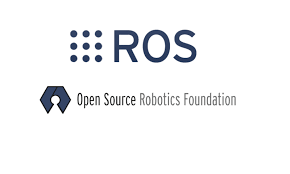
\includegraphics[width=6cm]{./pic/ros-intro.png}
		}
		\subfigure{
			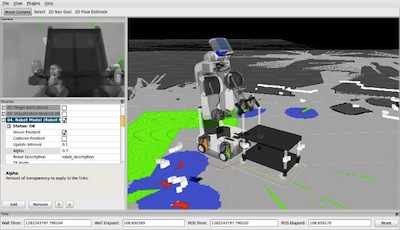
\includegraphics[width=8cm]{./pic/ros-screenshot.jpg}
		}
		\caption{ROS仿真环境}
	\end{figure}

	ROS的首要设计目标是在机器人研发领域提高代码复用率。ROS是一种分布式处理框架,这使可执行文件能被单独设计,并且在运行时松散耦合。这些过程可以封装到数据包(Packages)和堆栈(Stacks)中,以便于共享和分发。ROS还支持代码库的联合系统。使得协作亦能被分发。这种从文件系统级别到社区一级的设计让独立地决定发展和实施工作成为可能。上述所有功能都能由ROS的基础工具实现。
	
	为了实现“共享与协作”这一首要目标,人们制订了ROS架构中的其他支援性目标:
	
	\begin{itemize}
		\item 轻量级:ROS是设计得尽可能方便简易,不必替换主框架与系统即可用于其他机器人软件框架中。
		
		\item 语言独立性:ROS框架很容易在任何编程语言中执行。目前已经能在Python和C++中顺利运行,同时添加有Lisp、Octave和Java语言库。
		
		\item 测试简单:ROS有一个内建的单元/组合集测试框架,这使得集成调试和分解调试很容易。
		
		\item 扩展性:ROS适合于大型实时系统与大型的系统开发项目。
	\end{itemize}

	\subsection{Unity游戏引擎}
	Unity 是一套跨平台的游戏引擎,可用于开发 Windows、MacOS、Linux 平台的单机游戏,或是 iOS、Android 移动设备的游戏。Unity 也可开发支持 WebGL 技术的网页游戏,或 PlayStation、XBox、Wii 主机上的游戏。目前Unity被广泛应用于虚拟现实应用的开发,是虚拟现实技术栈中不可或缺的一部分。
	
	Unity 支持 PhysX 物理引擎、粒子系统,并且提供网络多人连接的功能,无需学习复杂的编程语言,匹配游戏制作上的各项需求。Unity 的推出降低游戏开发的门槛,即使是个人或小型团队制作游戏也不再是梦想。对于游戏公司而言,选择使用 Unity 引擎也可以缩短游戏的开发时间。
	
	Unity 类似于Director,Blender,Virtools或Torque Game Builder等利用交互的图型化开发环境为首要方式的软件其编辑器运行在Windows和Mac OS X下,可发布游戏至Windows、Wii、OSX或iOS平台。也可以利用Unity web player插件发布网页游戏,支持Mac和Windows的网页浏览。它的网页播放器也被Mac widgets所支持。Unity3D是一个用于创建诸如三维电子游戏、建筑可视化、实时三维动画等类型互动内容的综合型创作工具。
	\begin{figure}[h]
		\centering
		\subfigure{
			
\includegraphics[width=6cm]{./pic/unity-logo.jpg}
		}
		\subfigure{
			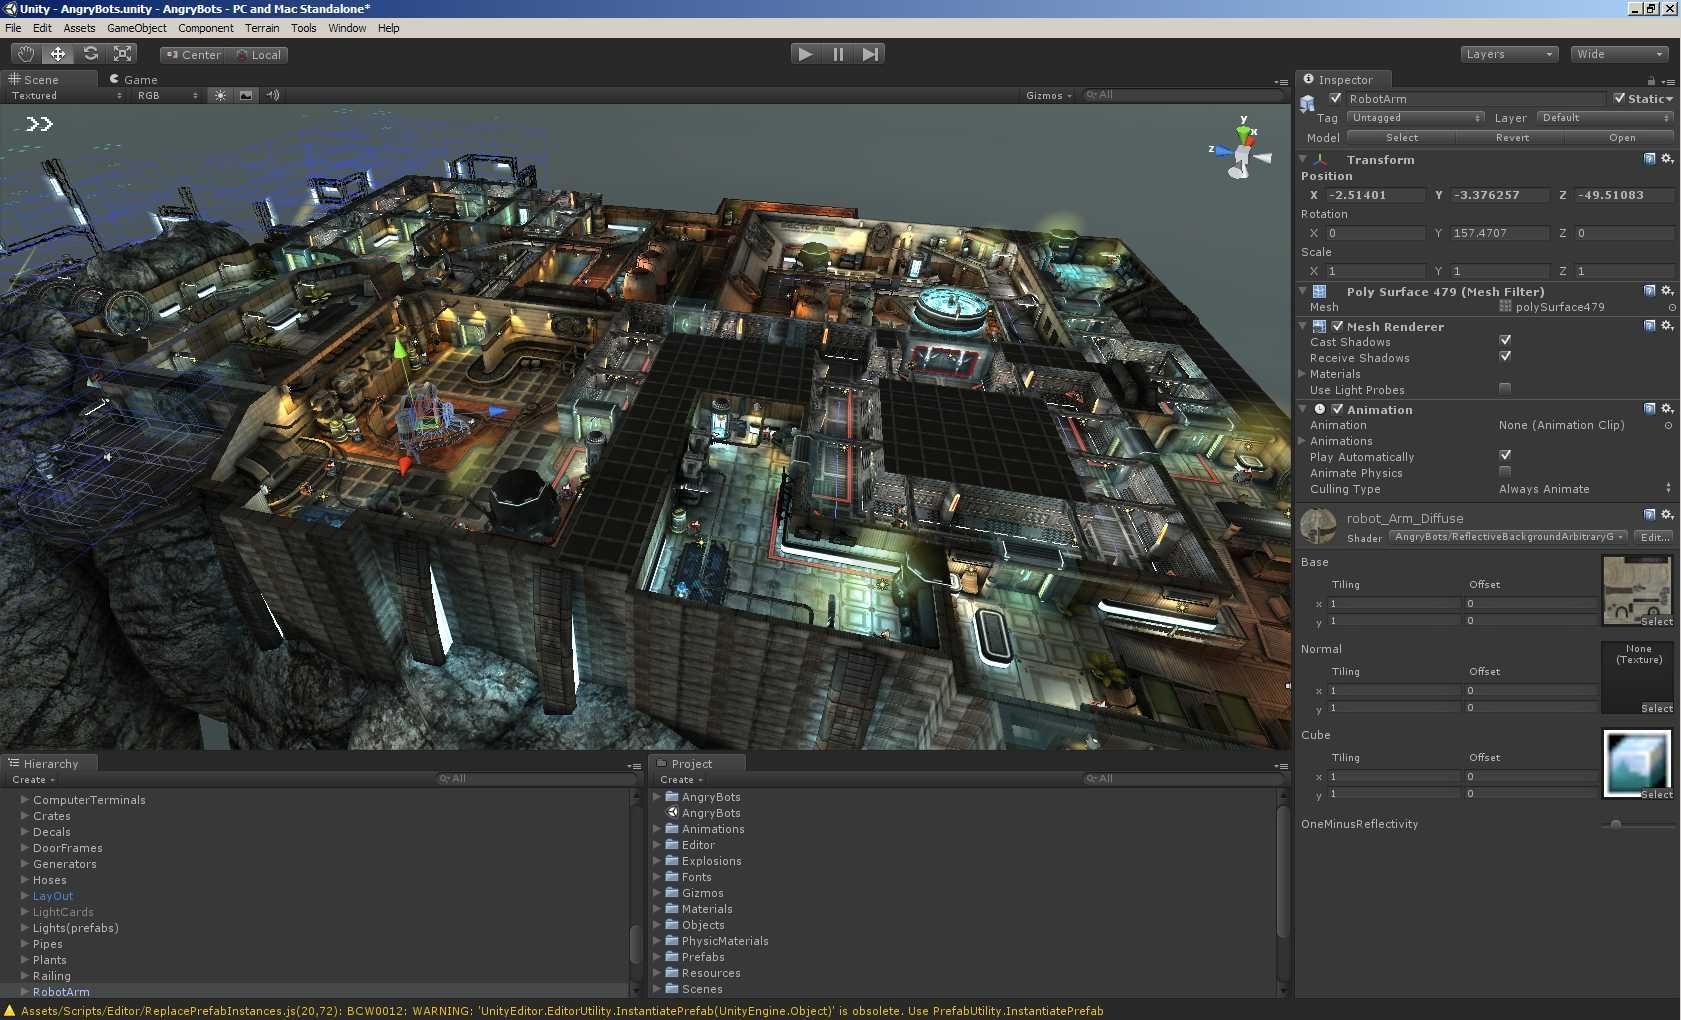
\includegraphics[width=8cm]{./pic/unity.jpg}
		}
		\caption{ROS仿真环境}
	\end{figure}

	\subsection{三者特性对比}
	严格来说,Unity的主要用途是游戏开发,但是得益于其优异的物理仿真性能,将其用于强化学习算法的训练也并非不可能。表\ref{compare}将Unity与Gym和ROS的特性进行了对比,可以看到Gym由于专注于为学术界提供标准,其自定义性并不强,而ROS则为工业界而生,专业性和复杂度都相当高,其功能大而全,而Unity则很好地平衡了两者的优缺点,所以将Unity平台于强化学习算法结合相当值得一试。
	
	\begin{table}[h]
		\caption{Gym、ROS、Unity三者特性对比}
		\label{compare}
		\begin{tabular}{cccccc}
			\toprule[1.5pt]
			架构 & 复杂度 & 易用性 & 物理引擎 & 3D模型导入 & 专业性 \\
			\hline
			Gym & 低 & 高 & 2D & 不支持 & 高 \\
			
			ROS & 高 & 低 & 3D & 支持 & 高 \\
			
			Unity & 低 & 高 & 2D/3D & 支持 & 中 \\ 
			\bottomrule[1.5pt]
		\end{tabular}
	\end{table}

	\section{PPO算法的具体实现}
	\begin{figure}[h]
		\centering
		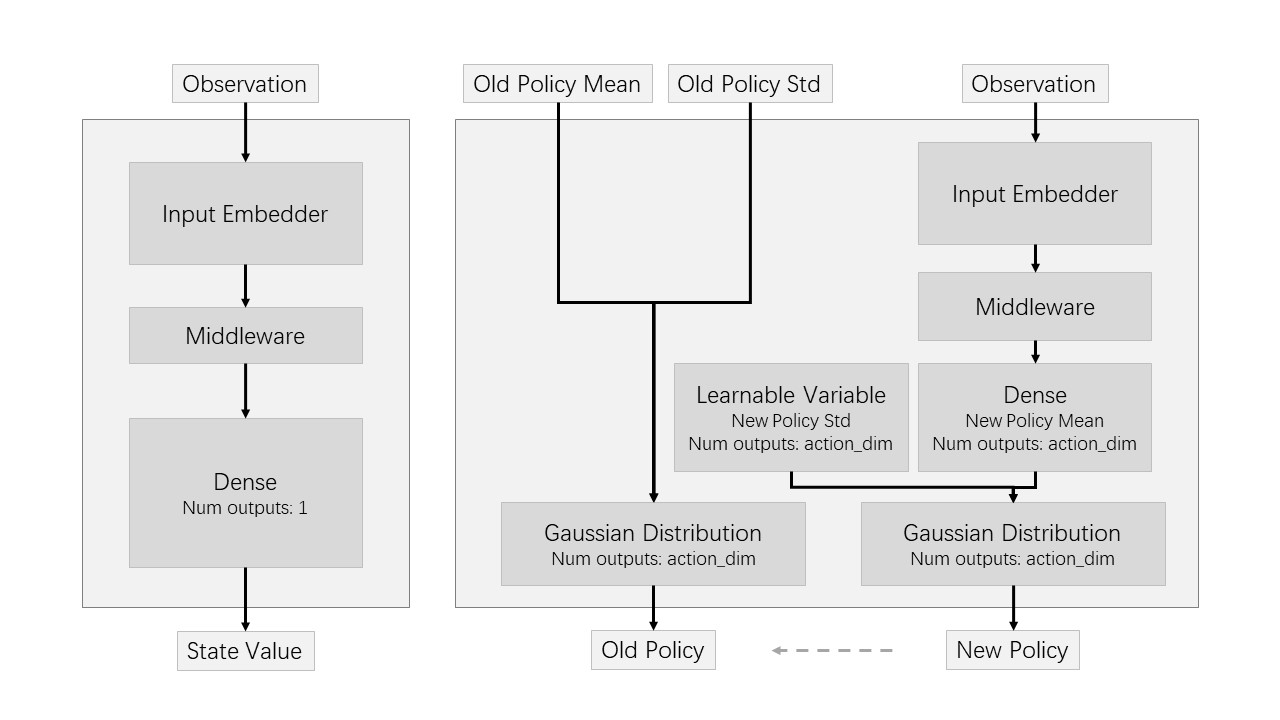
\includegraphics[width=14cm]{./pic/ppo.jpg}
		\caption{PPO网络结构}
		\label{ppofig}
	\end{figure}
	根据\ref{ppo}节所示的近端策略优化算法过程,搭建图\ref{ppofig}所示的网络。其中状态值函数采用一个全连接网络进行模拟,中间层节点为100个:
	\begin{lstlisting}
self.state_input = tf.placeholder(tf.float32, [None, S_DIM], 'state')
dense = tf.layers.dense(self.state_input, 100, tf.nn.relu)
self.value = tf.layers.dense(dense, 1) # 值函数的近似网络
	\end{lstlisting}
	同样地,策略网络也使用了类似的结构,但是由于强化学习中的策略是一个概率分布,所以用均值(mean)和方差(std)来描述该分布,其均值和方差均使用包含200个节点的全连接网络进行模拟:
	\begin{lstlisting}
dense = tf.layers.dense(self.state_input, 200, tf.nn.relu, trainable=True)
mu = A_BOUND * tf.layers.dense(dense, A_DIM, tf.nn.tanh, trainable=True)
sigma = tf.layers.dense(dense, A_DIM, tf.nn.softplus, trainable=True)
pi_norm_distribution = Normal(loc=mu, scale=sigma)
	\end{lstlisting}
	然后根据算法\ref{al2}中的$J_{PPO}(\theta)$和$L_{CLIP}(\phi)$确定行动者和评价者网络的损失函数,再定义其优化方式即可。
	\begin{lstlisting}
self.critic_loss = tf.reduce_mean(tf.square(self.advantage))
self.critic_train_op = tf.train.AdamOptimizer(LR).minimize(self.critic_loss)
self.actor_loss = - tf.reduce_mean(tf.minimum(surrogate, tf.clip_by_value(pi_ratio, 1 - EPSILON, 1 + EPSILON) * self.advantage_input))
self.actor_train_op = tf.train.AdamOptimizer(LR).minimize(self.actor_loss)
	\end{lstlisting}
	本小节仅列出了关键部分网络部分的代码,完整代码见附录部分。
	
	\section{二维机械臂环境中的PPO算法实践}
	为了验证和优化上小节实现的PPO算法,本节将搭建一个二维的简易机械臂环境,并将PPO算法集成到该环境中,然后进行训练,对其训练效果进行评估。之后再使用各种优化方法对算法进行优化,为下一步在Unity环境中仿真奠下基础。
	\subsection{架构设计}
	首先需要构建2D机械臂环境,在此选用python下的一个2D图形引擎pyglet。OpenAI的gym环境的接口经过了历次迭代已经十分成熟了,因此本节的机械臂环境的接口将按照gym风格进行封装。
	\begin{figure}[h]
		\centering
		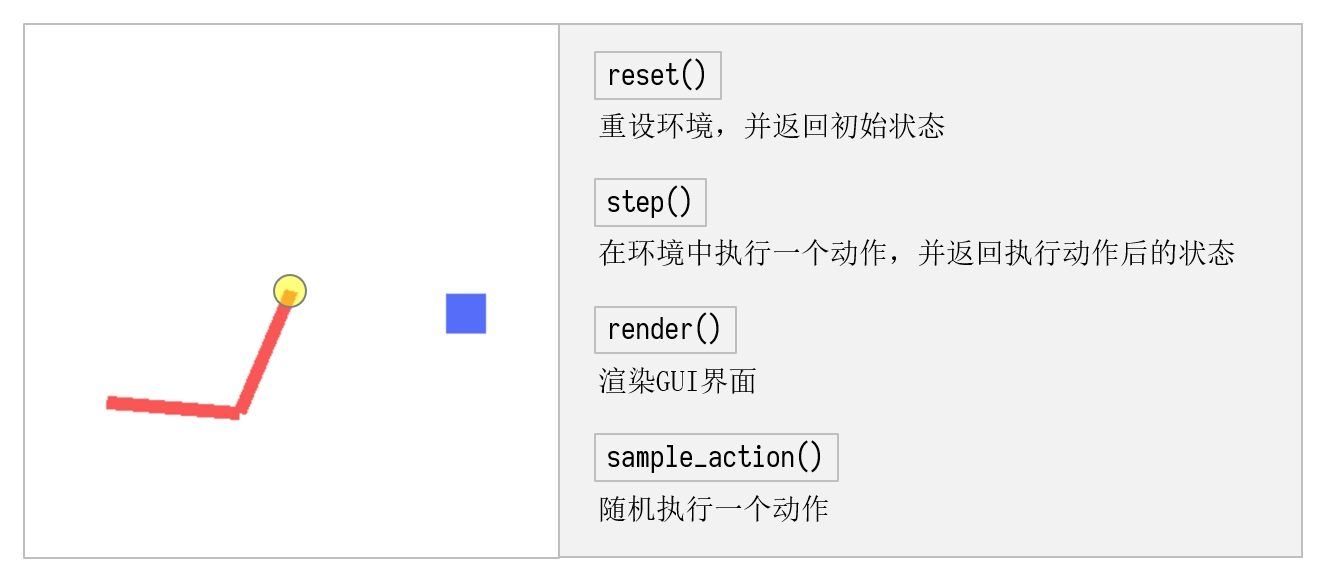
\includegraphics[width=14cm]{./pic/2darm.jpg}
		\caption{二维机械臂环境}
		\label{2darm}
	\end{figure}
	图\ref{2darm}展示了该机械臂环境的接口,这是一个简单的两关节机械臂,围绕着图像中心的固定点旋转,它可以接受一个二维动作向量$(angle_1,angle_2)$,分别表示了两个关节在当前状态应当设定的角速度,每次执行动作之后,环境便返回一个动作向量$(hasOnPoint,arm1_x,arm1_y,arm2_x,arm2_y,p_x,p_y)$,分别表示机械臂末端是否已与目标点重合、机械臂一关节尾端坐标、机械臂二关节尾端坐标,目标点坐标\footnote{此环境中返回的坐标值均是经过归一化后的坐标值,归一化公式:$norm(x)=\frac{x}{width\ of\ window}, norm(y)=\frac{y}{height\ of\ window}$。例如默认窗口宽高为$400\times500$,坐标值为$(200,300)$,则返回坐标值为$(0.5,0.6)$。}。也就说,该环境包含了2维度的动作空间和7维度的状态空间,这意味着PPO网络的输入与输出也要设置为对应的值。
	
	\begin{figure}[h]
		\centering
		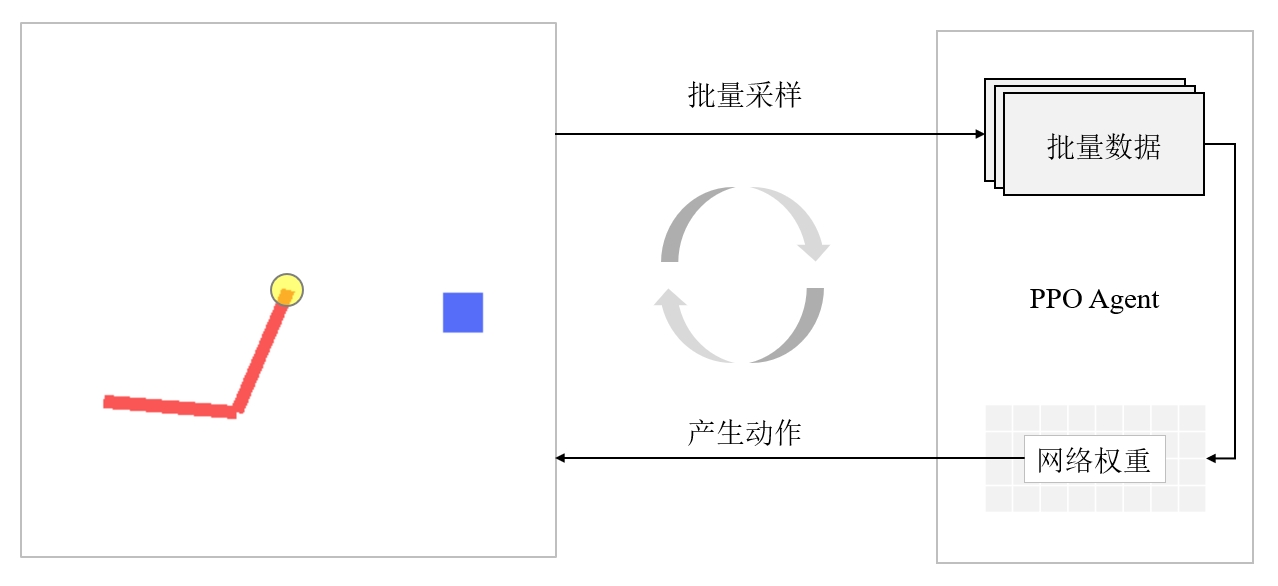
\includegraphics[width=14cm]{./pic/2darm-ppo.jpg}
		\caption{二维机械臂环境中集成PPO算法}
		\label{2darm-ppo}
	\end{figure}

	图\ref{2darm-ppo}展示了PPO算法与该机械臂环境的集成架构,由于该机械臂环境直接采用python中的一个GUI框架渲染而成,所以PPO可以直接像调用函数一样在训练时与该环境实时交互,这一点与gym环境的使用是类似的。就如算法\ref{al2}中所示,在训练时,PPO算法会先从环境中执行$N$次动作,这些动作对应的状态整合之后便作为网络权重训练的批数据,在实际训练时,使用Adam优化器对策略网络和值网络进行优化,每轮优化轮次为$M$,优化完成后进入下一轮采样-优化的循环,直至训练结束。
	\subsection{实验结果}
	\subsubsection{两种目标函数效果对比}\label{sec:kl_vs_clip}
	上文\ref{ppocontent}节提到了PPO算法有两种可选的目标函数,一种是带惩罚项的动态$\lambda$调整目标函数$L_{BL}(\theta)$,另一种是使用裁剪概率比率限制策略更新幅度的目标函数$L_{CLIP}(\theta)$。本节主要对两种目标函数的效果进行对比。
	\begin{figure}[h]
		\centering
		\subfigure[两者的reward对比]{
			\includegraphics[width=7cm]{./pic/kl-vs-clip.pdf}
		}
		\subfigure[$L_{BL}(\theta)$中$\lambda$随着训练进行不断变化]{
			\includegraphics[width=7cm]{./pic/kl-lambda.pdf}
		}
		\caption{}
		\label{kl-vs-clip}
	\end{figure}
	
	从图\ref{kl-vs-clip}(a)可以看出,训练前期$L_{CLIP}(\theta)$的reward上升速度稍快一些,而且后期$L_{CLIP}(\theta)$的reward更加稳定,虽然$L_{BL}(\theta)$在后期的平均效果要更好,但是波动幅度很大,由\ref{kl-vs-clip}(b)可知,超参数$\lambda$在训练后期波动很大,这是因为后期的策略更新幅度一般偏大,从而需要较大的惩罚项来限制这种波动。
	
	\ref{ppocontent}节中指出$L_{CLIP}(\theta)$的数据效率要比$L_{BL}(\theta)$更高,但由于本节搭建的二维机械臂环境比较简单,状态空间与动作空间维度都很小,$L_{CLIP}(\theta)$的优势并没有表现得特别突出,所以后文将继续对两者进行比较。
	
	\begin{figure}[h]
		\centering
		\subfigure[$L_{BL}(\theta)$中超参数$KL_{target}$对效果的影响]{
			\includegraphics[width=7cm]{./pic/kl_target.pdf}
		}
		\subfigure[$L_{CLIP}(\theta)$中超参数$\epsilon$对效果的影响]{
			\includegraphics[width=7cm]{./pic/clip_epsilon.pdf}
		}
		\caption{两种目标函数中超参数对训练效果的影响}
		\label{hyperparams}
	\end{figure}
	此外两目标函数中均存在超参数,其中$L_{BL}(\theta)$中的$KL_{target}$直接影响了$\lambda$的动态调整过程,但如图\ref{hyperparams}(a)所示,该参数对训练结果的影响并不大;而$L_{CLIP}(\theta)$中的裁剪比率阈值$\epsilon$则更加敏感,从图\ref{hyperparams}(b)可以看出,随着阈值$\epsilon$的增大,后期的训练效果变得愈发不稳定,这是因为阈值$\epsilon$限制了策略更新的幅度,阈值$\epsilon$越大,策略更新幅度就越大,就越有可能训练出“坏”策略\footnote{策略更新幅度过大造成的影响详见\ref{ppocontent}节},因此,选用$L_{CLIP}(\theta)$作为目标函数时,应当采用较小的$\epsilon$值。
	
	\subsubsection{探究随机化目标点对训练结果的影响}
	在前面的训练过程中,目标点的选取始终是固定的,每次环境重置(reset)后会重新随机放置机械臂的位置,这种做法存在一个弊端,由于环境返回的状态向量也包含了目标点的坐标,如果每次目标点位置都固定,则所有的数据后两维均是相同的。于是考虑在每次初始化时,随机选择目标点的位置。
	
	图\ref{fixed-point}展示了随机选择目标点对训练效果的影响,由图\ref{fixed-point}(c)可以看到,随机初始化会大幅减缓网络效果的提升,这是因为每次训练都要重新对新的目标点进行优化,网络需要收集更多数据后才能取得比较好的效果,可以看到,600个训练周期以后,两者的训练效果便相差无几。
	
	随机初始化会大大提高网络的的泛化能力,通过对引入随机初始化前后的模型进行测试发现,引入后机械臂的移动更加顺滑,任务失败率也大大地降低了。
	\begin{figure}[h]
		\centering
		\subfigure[初始化时,机械臂随机摆放,目标点固定]{
			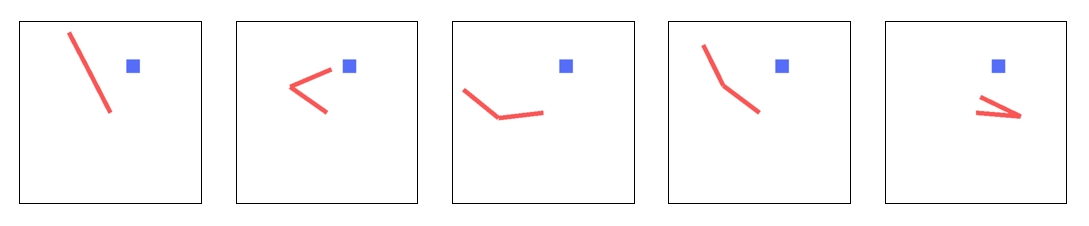
\includegraphics[width=14cm]{./pic/fixed-point.jpg}
		}
		\subfigure[初始化时,机械臂随机摆放,目标点随机出现]{
			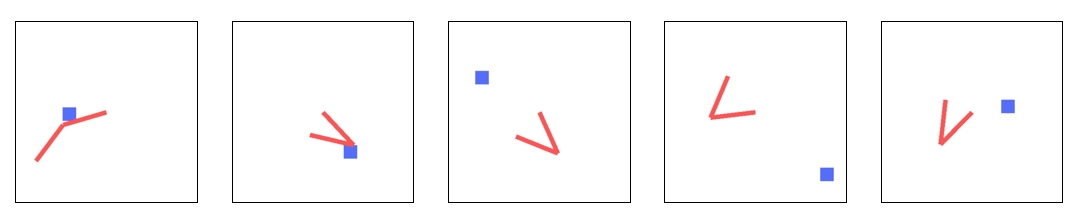
\includegraphics[width=14cm]{./pic/random-point.jpg}
		}
		\subfigure[两种初始化方式对训练效果的影响对比]{
			\includegraphics[width=14cm]{./pic/should_random_target.pdf}
		}
		\caption{目标点随机初始化的影响}
		\label{fixed-point}
	\end{figure}
	\subsubsection{探究批规范化对训练结果的影响}
	批规范化(Batch Normalization)\cite{Ioffe2015Batch}已被广泛证明可以很好解决神经网络训练过程中“梯度消失”的问题,并且可以显著地改善网络效果。本节将讨论在PPO算法的近似网络中添加批规范化对训练效果的影响。
	
	PPO算法中的行动者近似网络的优化会依赖优势函数$\hat{A_t}=\sum_{t'>t}\gamma^{t'-t}r_{t'}-V_\phi(s_t)$,即优势函数与状态向量构成了行动者近似网络的输入,于是考虑对优势函数进行规范化处理:
	\begin{equation}
		\label{eq30}
		Norm(\hat{A_t})=\frac{\hat{A_t}-E(\hat{A_t})}{\sigma(\hat{A_t})}
	\end{equation}
	\begin{figure}[h]
		\includegraphics[width=14cm]{./pic/should_norm_advantage.pdf}
		\caption{规范化优势评价指标对训练效果的影响}
		\label{norm}
	\end{figure}
	由图\ref{norm}可以看出,引入规范化会使前期的训练稍慢,同时后期训练出的模型表现会更加稳定。
	\subsubsection{进一步优化}
	为了进一步优化训练效果,本节将对模型中的更多参数进行讨论。在前面的实验过程中,发现每次训练时间耗时略长,于是考虑对实验的时间开销进行优化。
	
	\begin{table}[htbp]
		\centering
		\caption{影响运行时间的参数TOP10}
		\begin{tabular}{cccl}
			\toprule[1.5pt]
			参数 & 值 & 每千次训练耗时(s) & 备注\\
			\hline
			$EP_{LEN}$ & 100   & 94.06173 & 每轮训练次数\footnotemark[1] \\
			Batch Size & 128   & 117.7748 & 批采样数据大小\footnotemark[2] \\
			Batch Size & 64    & 140.2311 & 批采样数据大小 \\
			$KL_{target}$ & 0.1   & 147.4605 & $L_{BL}(\theta)$中的$
			\lambda$约束\footnotemark[3] \\
			$KL_{target}$ & 0.05  & 163.9781 & $L_{BL}(\theta)$中的$
			\lambda$约束\\
			Batch Size & 32    & 170.9606 & 批采样数据大小\\
			$M$ & 10    & 171.3174 & 行动者网络更新次数 \footnotemark[3]\\
			$\epsilon$ & 0.5   & 171.4027 & 裁剪阈值 \footnotemark[3]\\
			$B$ & 10    & 171.5989 & 评价者网络更新次数 \footnotemark[3]\\
			\hline
			- & - & 225.4256 & 默认情况下的训练耗时,作为基准\\
			\bottomrule[1.5pt]
		\end{tabular}%
		\label{params-table}%
	\end{table}
	\footnotetext[1]{相当于算法\ref{al1}中的$N$}
	\footnotetext[2]{相当于算法\ref{al1}中的$T$}
	\footnotetext[3]{相当于算法\ref{al2}中的同名参数}
	
	表\ref{params-table}列出了算法中不同参数的取值对训练时间耗时的影响,可以看到,每轮训练次数$EP_{LEN}$和批采样数据量大小Batch Size极大地影响了训练时间,同时从图\ref{other-hyperparams}可以看到,当$EP_{LEN}$和Batch Size均取到理想值时,不会对训练结果产生影响。不仅如此,Batch Size设置为128时,在训练后期比其他参数都更稳定。
	
	注意到$\epsilon$设置为0.5时,也可以减少训练耗时,但前文\ref{sec:kl_vs_clip}一节中提到,增大$\epsilon$会使训练效果变差,所以不应对$\epsilon$进行变动。
	
	因此可以确定,参数$EP_{LEN}=100$以及Batch Size=128时,可以兼顾训练效果和时间开销。经测试,优化后每千次训练耗时缩短到了90s左右,速度提升了约170\%。

	\begin{figure}[h]
		\centering
		\subfigure[批采样数据量大小对训练结果的影响]{
			\includegraphics[width=7cm]{./pic/BATCH.pdf}
		}
		\subfigure[每批次训练次数对训练结果的影响]{
			\includegraphics[width=7cm]{./pic/EP_LEN.pdf}
		}
		\caption{其他参数对训练效果的影响}
		\label{other-hyperparams}
	\end{figure}
	\subsection{总结}
	本章节主要描述了在二维机械臂环境中的PPO算法实践过程,首先在pyglet图形引擎基础上搭建了一个包含7维度状态空间和2维度动作空间的简单机械臂环境,然后在此机械臂环境上进行了大量实验,对前文中提到的两种目标函数,以及算法中的参数对实验结果的影响进行了检验。实验结果表明,基于裁剪概率比率的目标函数$L_{CLIP}(\theta)$比基于动态惩罚项的目标函数$L_{BL}(\theta)$拥有更稳定的表现,其次初始环境参数的随机化以及对优势评价指标规范化同样可以提高模型稳定性,最后对模型中的其他参数进行了调优,使得模型训练的时间开销大幅减少。
	
	本章节的主要目的是为后续在更复杂的三维环境中实践PPO算法奠下基础,为之后的模型优化和架构设计积累经验。
	
	\section{三维机械臂环境中的PPO算法实践}
	\subsection{架构设计}
	[TODO]
	\subsection{实验结果}
	[TODO]
	\subsection{总结}
	[TODO]
	
	\chapter{全文总结与展望}
	\section{全文总结}
	[TODO]
	
	\section{后续工作展望}
	[TODO]
	
	\thesisacknowledgement
	[TODO]
	
	
	\thesisloadbibliography[nocite]{reference}
	
	%
	% Uncomment following codes to load bibliography database with native
	% \bibliography command.
	%
	% \nocite{*}
	% \bibliographystyle{thesis-uestc}
	% \bibliography{reference}
	%
	
	\thesisappendix
	%\lstinputlisting{../project/simply_PPO.py}
	
	\thesistranslationoriginal

	\begin{figure}[h]
		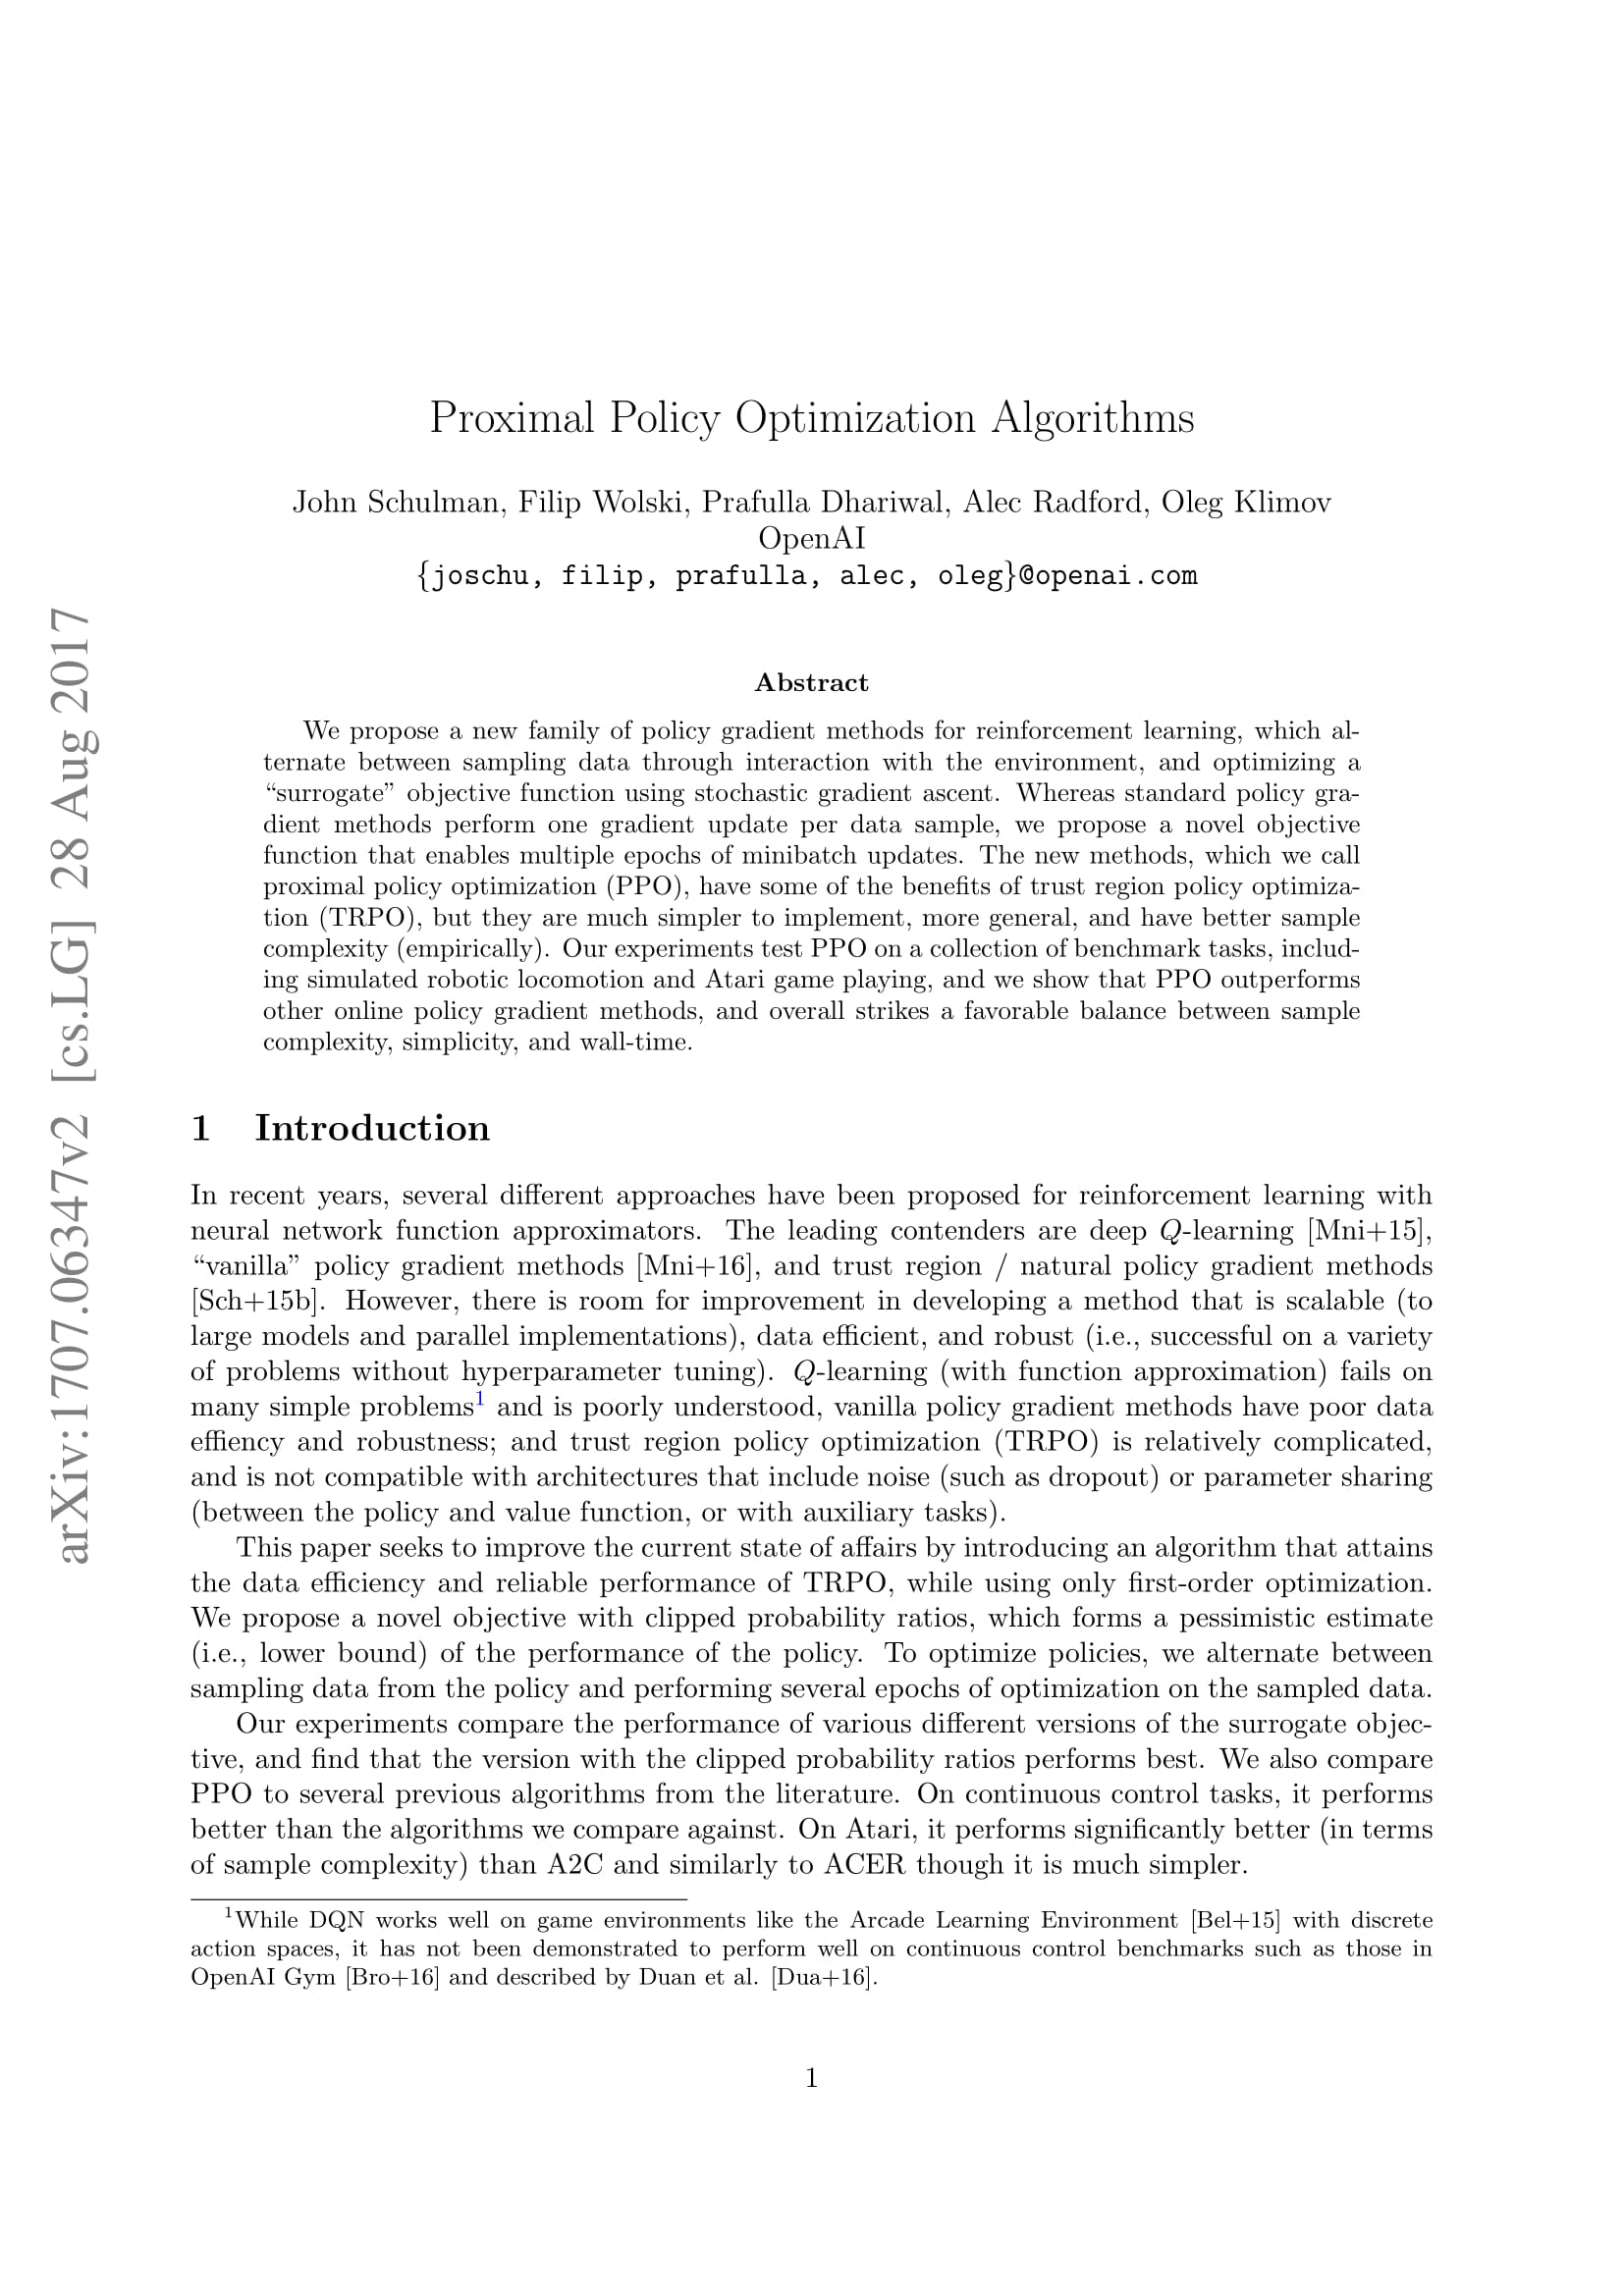
\includegraphics[width=13cm]{./pic/ProximalPolicyOptimizationAlgorithms-01.jpg}
	\end{figure}
	\begin{figure}[h]
		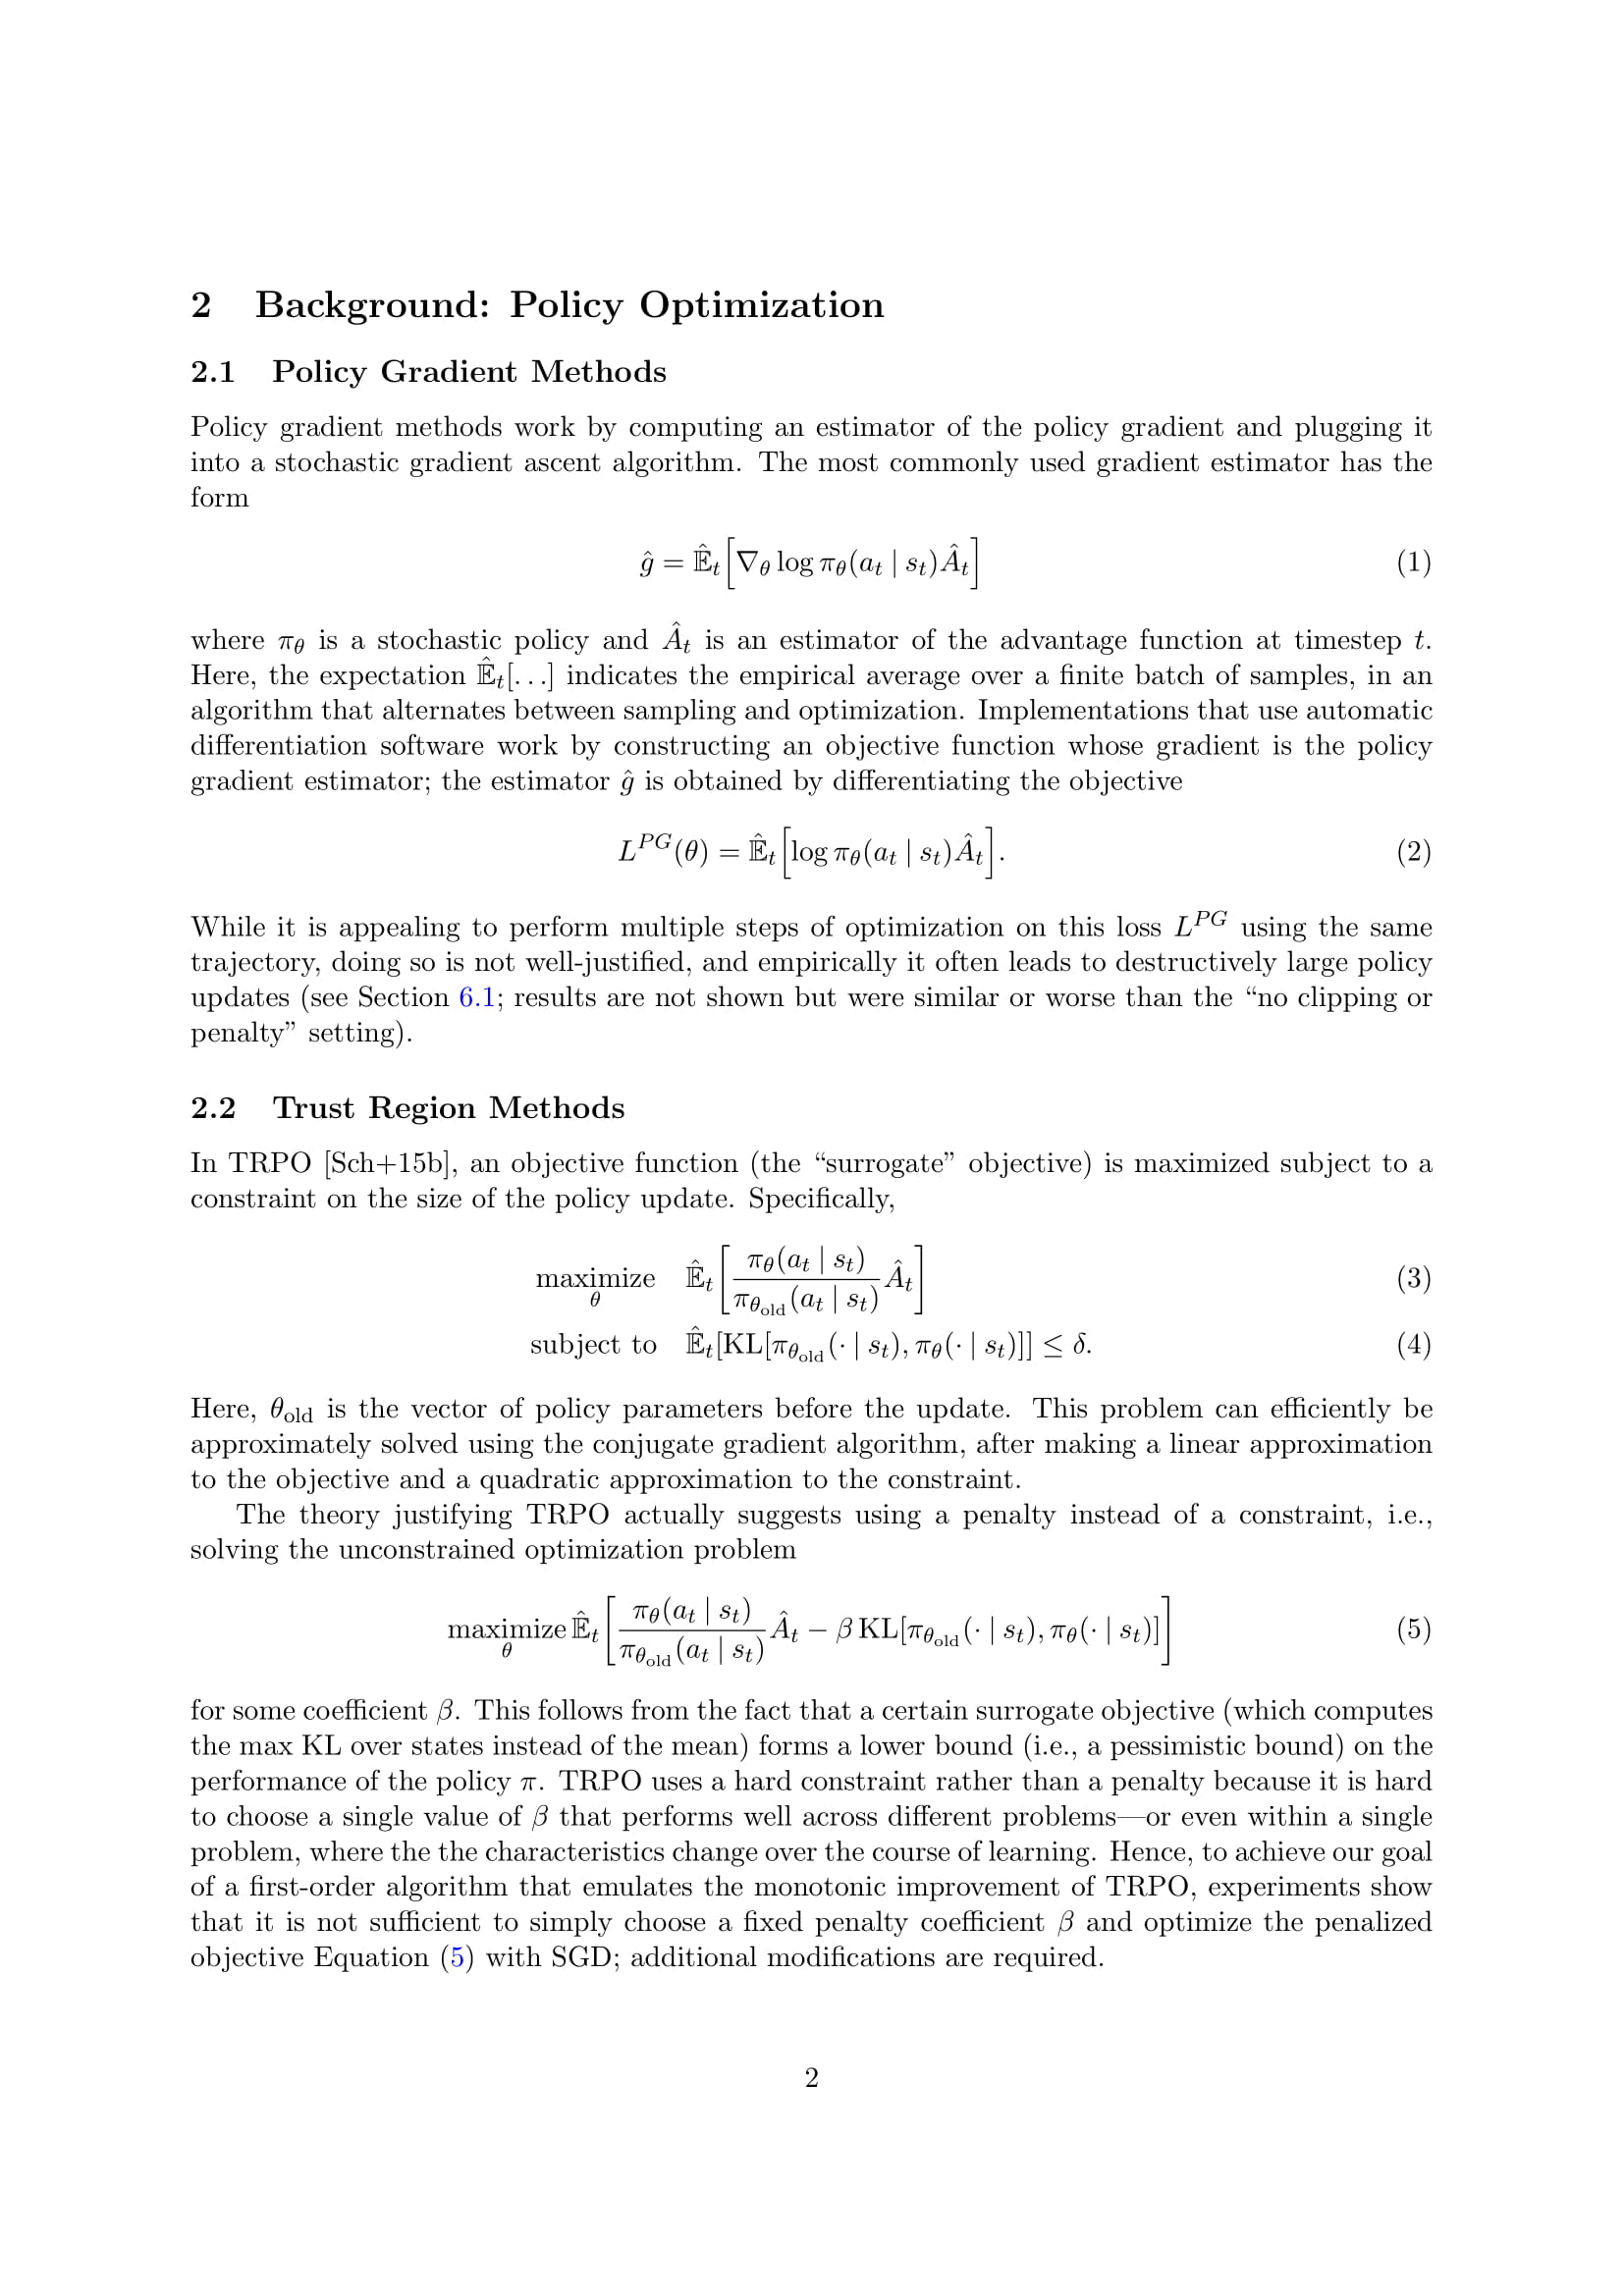
\includegraphics[width=14cm]{./pic/ProximalPolicyOptimizationAlgorithms-02.jpg}
	\end{figure}
	
	\thesistranslationchinese
	\begin{center}
		\textbf{\large 近端策略优化算法}
	\end{center}

	\section{摘要}
	本文提出一种新的基于策略梯度的强化学习算法,此算法交替地执行数据采样和策略优化过程,在数次与环境交互并取得批量采样数据之后,此算法会使用随机梯度下降法优化“代理”目标函数,如此循环往复。传统的策略梯度算法每采样一次数据就会执行一次梯度更新,我们提出了一种新的目标函数,可以采用多轮小批量数据进行梯度更新。我们提出的这种名为近端策略优化的算法,基于置信域策略优化算法发展而来,但与之相比更易于实现、泛化能力更强以及拥有更好的采样复杂度。我们在多个基准测试任务上测试了该算法,包括仿真机械运动和雅达利游戏,并且发现该算法取得了相比于其他在线策略梯度算法更好的性能,在采样复杂度、朴素性和时间复杂度上取得了很好的平衡。
	
	\section{介绍}
	近些年,强化学习领域出现了多种基于神经网络近似的算法,其中最具代表性的算法有:深度Q学习[Mni+15]、普通策略梯度算法[Mni+16]和置信域策略梯度算法。然而,这些算法在可扩展性、效率和鲁棒性上还有很大的提升空间。Q学习(采用函数模拟的)不仅在很多简单任务上表现很差,而且可解释性很弱,普通策略梯度算法效率和鲁棒性都无法令人满意;而置信域策略优化算法相对来说太过复杂,并且无法很好地兼容包含噪声(如随机失活)或者包含参数共享结构(策略函数与值函数共享或者多任务参数共享)的架构。
	
	本文旨在提出一种比TRPO算法拥有更高的效率和更可靠的性能的仅使用了一阶优化函数的高效算法。我们提出的目标函数使用裁剪概率比率来评估策略性能的下界。为了优化策略,我们交替地批量采样数据并用这些数据优化目标函数。
	
	我们在实验中对比了多种版本的代理目标函数,并且发现使用裁剪概率比率的版本表现最好。同时,我们也将该算法与其他文献中的算法进行了对比。在连续空间任务上,该算法比竞争算法表现都好。而在雅达利游戏上,该算法远远超出了A2C的表现,并在更低的复杂度上取得了与ACER类似的成绩。
	
	\section{背景知识:策略优化理论}
	\subsection{策略梯度算法}
	策略梯度算法使用一个评价函数来评价策略梯度,并且使用随机梯度下降对该评价函数进行优化。最广泛使用的评价函数如式(\ref{teq1})所示。
	\begin{equation}
		\label{teq1}
		\hat{g}=\hat{E}_t[\nabla_\theta log\pi_\theta(a_t|s_t)\hat{A_t}]
	\end{equation}
	其中$\pi_\theta$是一个随机变量,表示策略(policy),而$\hat{A_t}$则是在时间步$t$时的优势评价指标。数学期望$\hat{E}_t$表示有限数量样本的经验平均值,它通常在数据采样和优化时变化。为了能够使用自动求导来解决问题,通常需要构造一个目标函数,这个目标函数的梯度便是策略梯度评价指标;评价指标$\hat{g}$可以通过对以下目标函数求导得到:
	\begin{equation}
		\label{teq2}
		L^{PG}(\theta)=\hat{E}_t[log\pi_\theta(a_t|s_t)\hat{A_t}]
	\end{equation}
	尽管我们希望损失函数$L^{PG}$在多步以后沿着同样的轨迹优化,但事实却并不如此,这种优化方式往往引起巨量的策略更新。
	
	\subsection{基于置信域的方法}
	在TRPO算法中,最大化目标函数时,使用策略更新的尺寸来约束,具体地,
	\begin{equation*}
	\label{teq3}
	\begin{aligned}
		& \underset{\theta}{\text{maximize}}& & \hat{E}_t[\frac{\pi_\theta(a_t|s_t)}{\pi_{\theta_{old}}(a_t|s_t)}\hat{A_t}]\\
		& \text{subject to }& &\hat{E}_t[KL[\pi_{\theta_{old}}(\cdot|s_t),\pi_\theta(\cdot|s_t)]]\leq \delta
	\end{aligned}
	\end{equation*}
	其中,$\theta_{old}$是更新前的策略参数向量。在对目标函数进行线性近似并对约束条件进行二阶近似后,这个问题可以使用共轭梯度算法来有效地解决。
	
	TRPO算法在进行策略调整时,没有使用惩罚项来代替约束。也就是说,求解包含系数$\beta$的非约束最优化问题
	\begin{equation}
		\label{teq4}
		\underset{\theta}{\text{maximize }} \hat{E}_t[\frac{\pi_\theta(a_t|s_t)}{\pi_{\theta_{old}}(a_t|s_t)}\hat{A_t}]-\beta KL[\pi_{\theta_{old}}(\cdot|s_t),\pi_\theta(\cdot|s_t)]
	\end{equation}
	该问题成立的前提是,存在这样一个事实:一个确定的代理目标函数(通过计算状态的KL散度而不是其平均值)形成了策略$\pi$的下界。TRPO选用一个强约束条件而不是惩罚项来求解最优化问题,这是因为很难确定一个能够在多种问题上都取得很好效果的$\beta$值——甚至在单一问题上也很难确定合适的$\beta$值。因此,为了达到我们使用一阶函数改进TRPO算法的目标,实践证明,简单地选取一个固定的系数$\beta$然后去优化惩罚目标式(\ref{teq4})是远远不够的,我们需要进行更多的改动。
\end{document}
